\documentclass[12pt,a4paper]{article}
 
\usepackage{float}
%für feststellen der figures und tables [H] dranschreiben
\usepackage{units}
%wird so benutzt: 
%\unit[value/Zahl]{dimension/Einheit} oder 
%\unitfrac[value/Zahl]{dimension/Einheit num/Zähler}{dimension/Einheit denum/Nenner} oder
%\nicefrac[fontcommand/Schriftart]{dimension/Einheit num/Zähler}{dimension/Einheit denum/Nenner}
\usepackage[left=2cm,right=2cm,top=2cm,bottom=2cm]{geometry}
\usepackage[utf8]{inputenc}
\usepackage[T1]{fontenc}
\usepackage{lmodern}
\usepackage[ngerman]{babel}
\usepackage{amsmath}
\usepackage{graphicx}

\usepackage{caption}
\usepackage{subcaption}
 
\title{Versuch EP1}
\author{Frederik Strothmann, Henrik Jürgens}
\date{\today}
%niemals zwei überschriften direkt übereinander schreiben, also immer mindestens in einem satz was sinnvolles unter jede überschrift schreiben (bei den versuchen z.B. das versuchsziel) 
\begin{document}
%deckblatt erstellen.
\maketitle
\newpage
\tableofcontents
\newpage

\section*{Vorgefertigte Skizzenausschnitte}




\begin{figure}[H] 
  \centering
    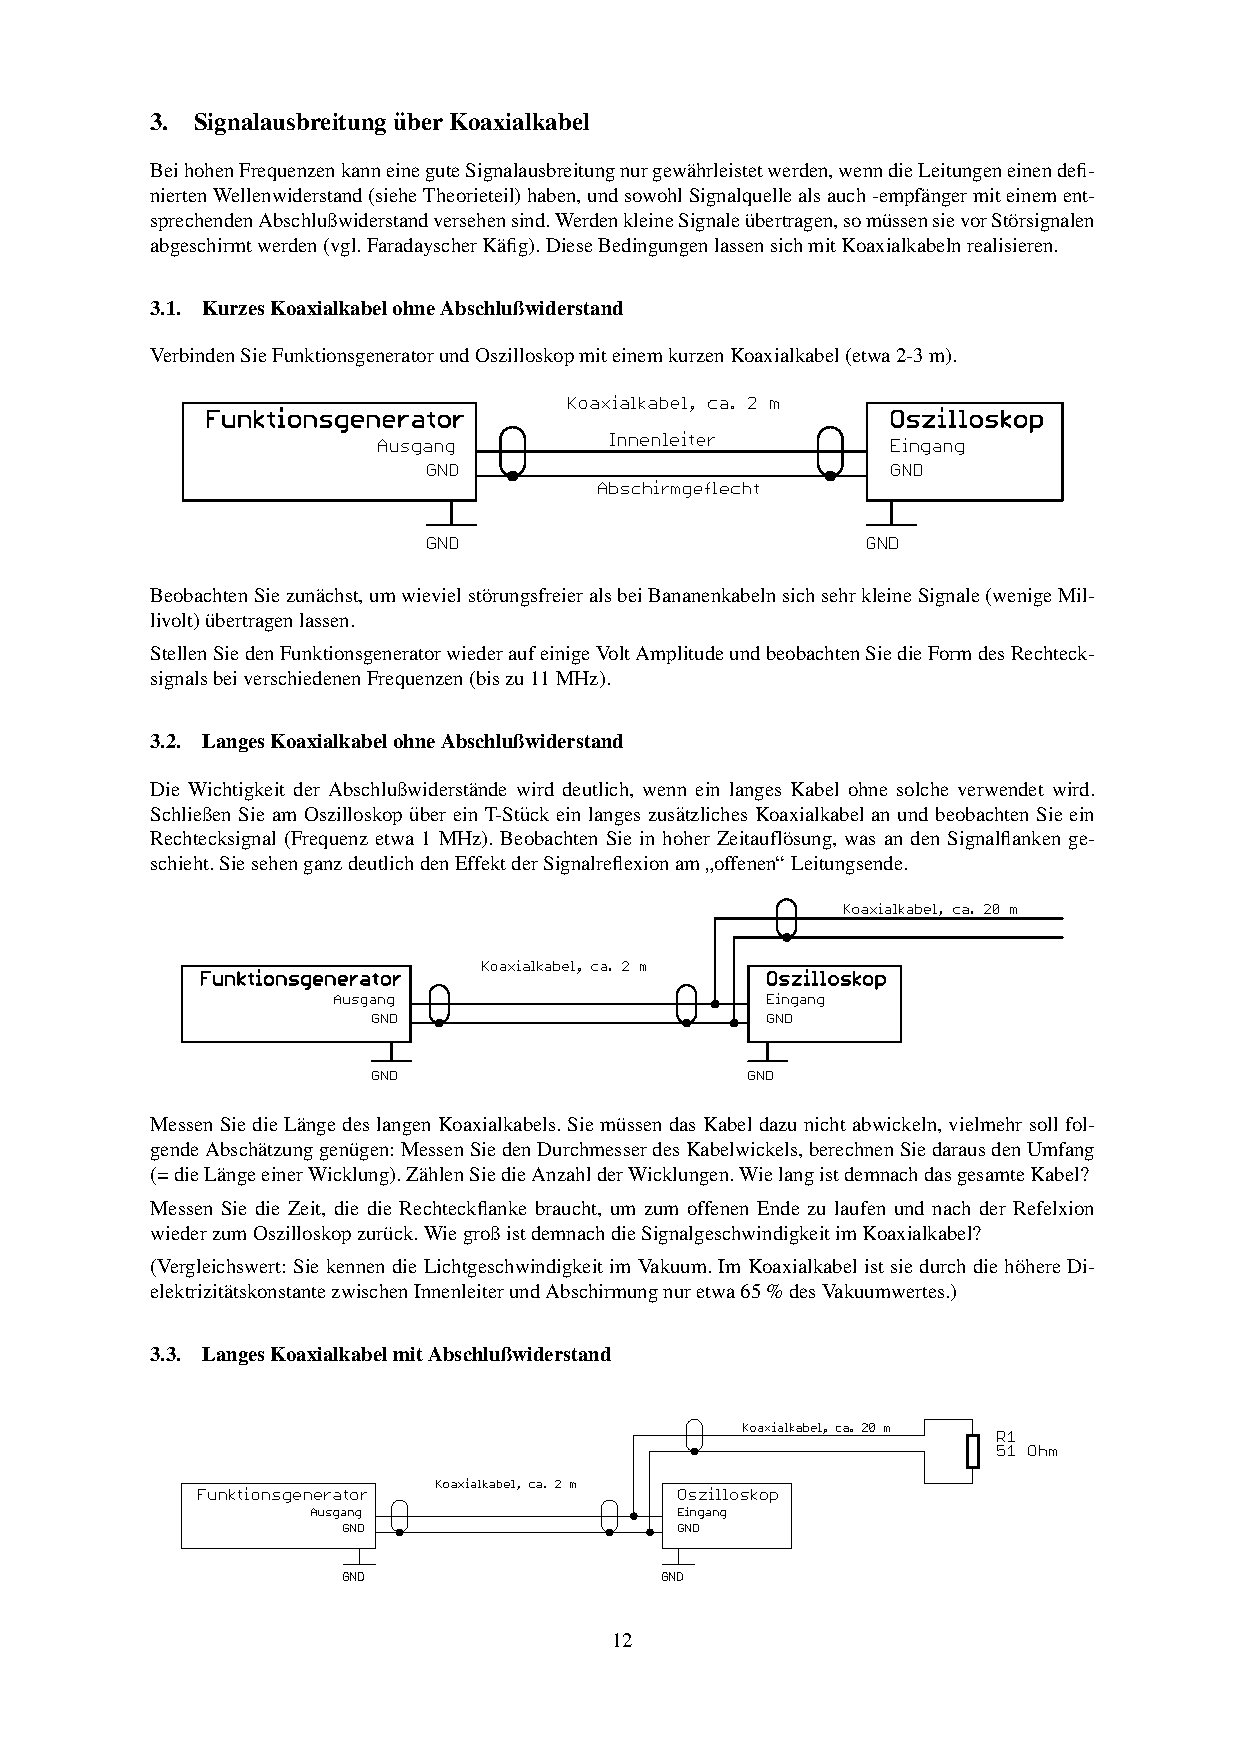
\includegraphics[trim = 10mm 200mm 10mm 65mm, clip, scale = 1]{3-3_3.pdf}
  	\caption[Schaltskizze einer Verbindung zwischen Funktionsgenerator und Oszilloskop, mit kurzem Koaxialkabel]{Schaltskizze einer Verbindung zwischen Funktionsgenerator und Oszilloskop, mit kurzem Koaxialkabel\footnotemark}
  \label{fig:3.1}
\end{figure}
\footnotetext{Abbildung entnommen von http://www.atlas.uni-wuppertal.de/$\sim$kind/ep1\_14.pdf Seite 12 am 19.10.2014}

\begin{figure}[H] 
  \centering
    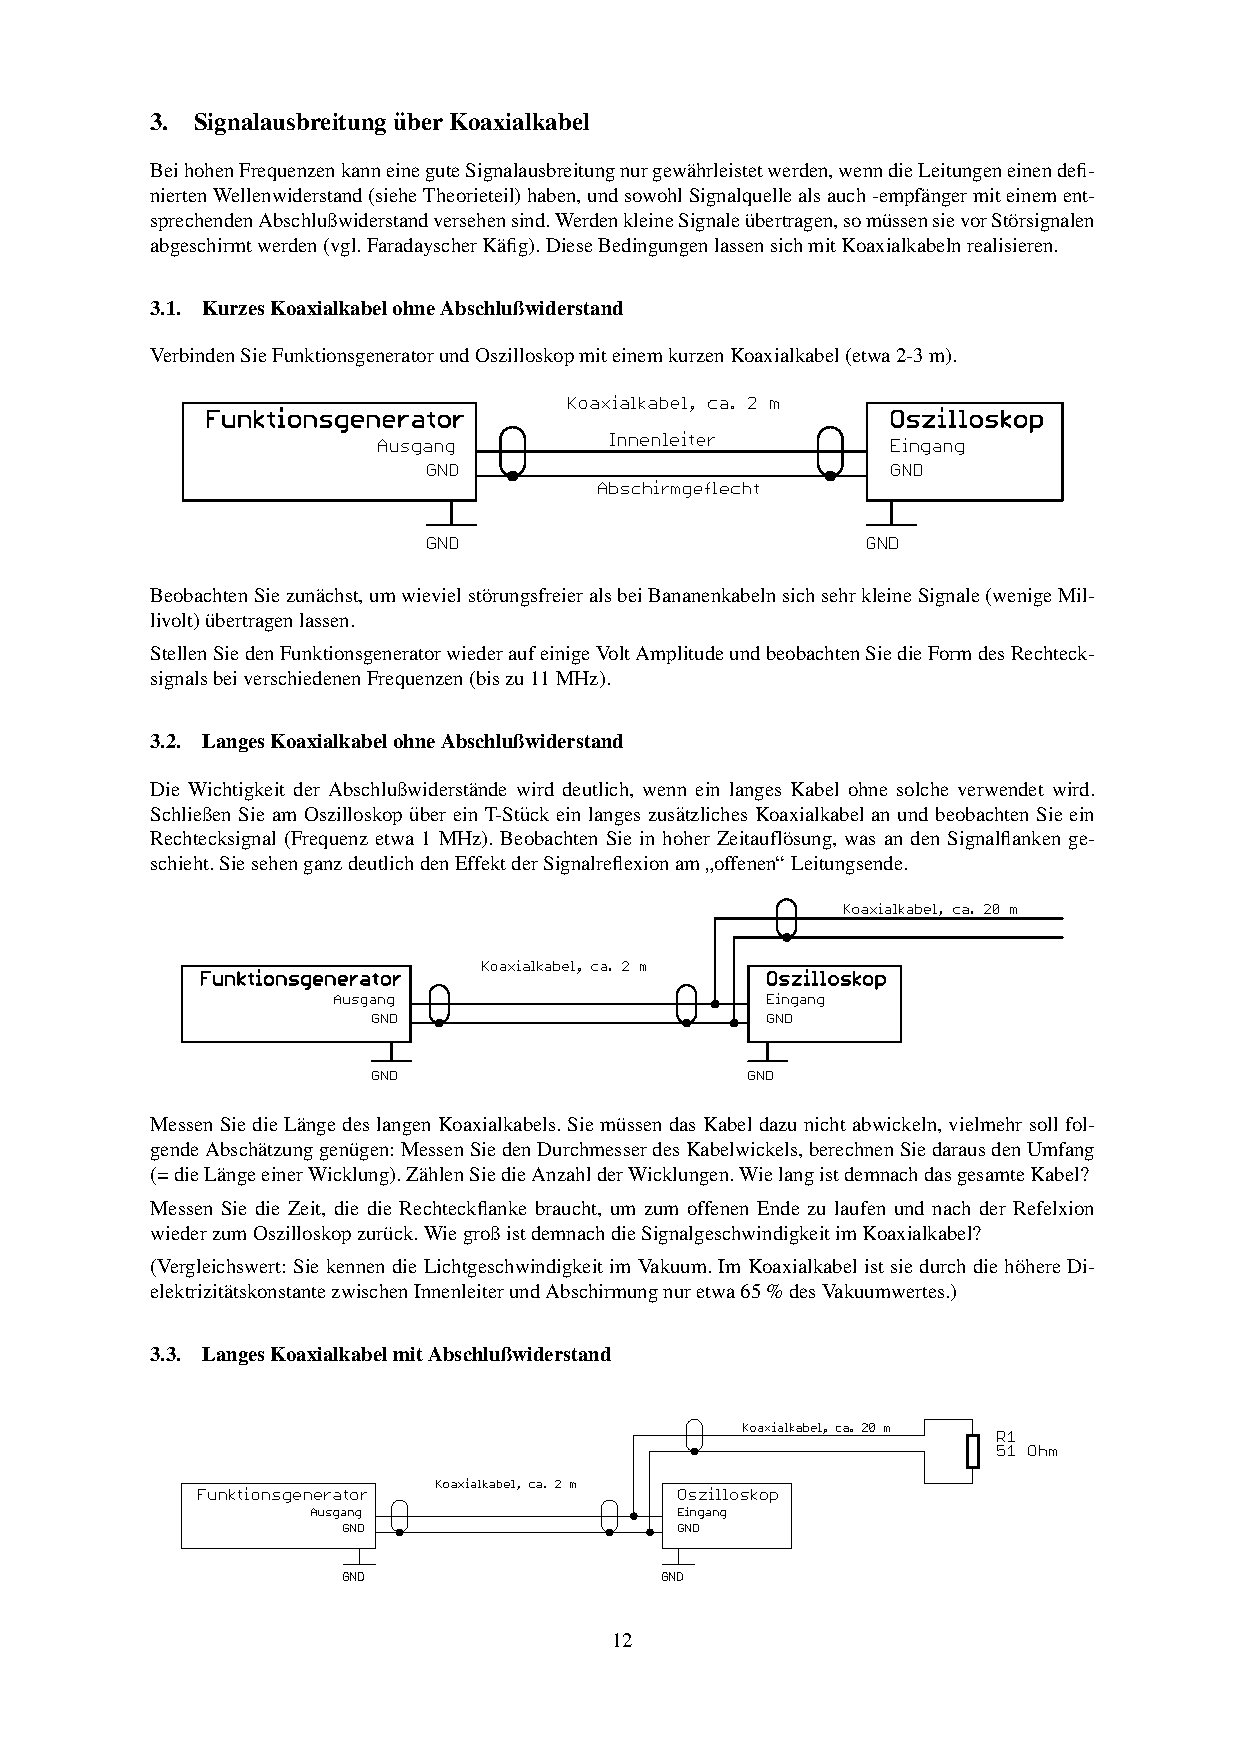
\includegraphics[trim = 10mm 110mm 10mm 150mm, clip, scale = 1]{3-3_3.pdf}
  	\caption[Schaltskizze einer Verbindung zwischen Funktionsgenerator und Oszilloskop, mit langem Koaxialkabel]{Schaltskizze einer Verbindung zwischen Funktionsgenerator und Oszilloskop, mit langem Koaxialkabel\footnotemark}
  \label{fig:3.2}
\end{figure}
\footnotetext{Abbildung entnommen von http://www.atlas.uni-wuppertal.de/$\sim$kind/ep1\_14.pdf Seite 12 am 19.10.2014}


\begin{figure}[H] 
  \centering
    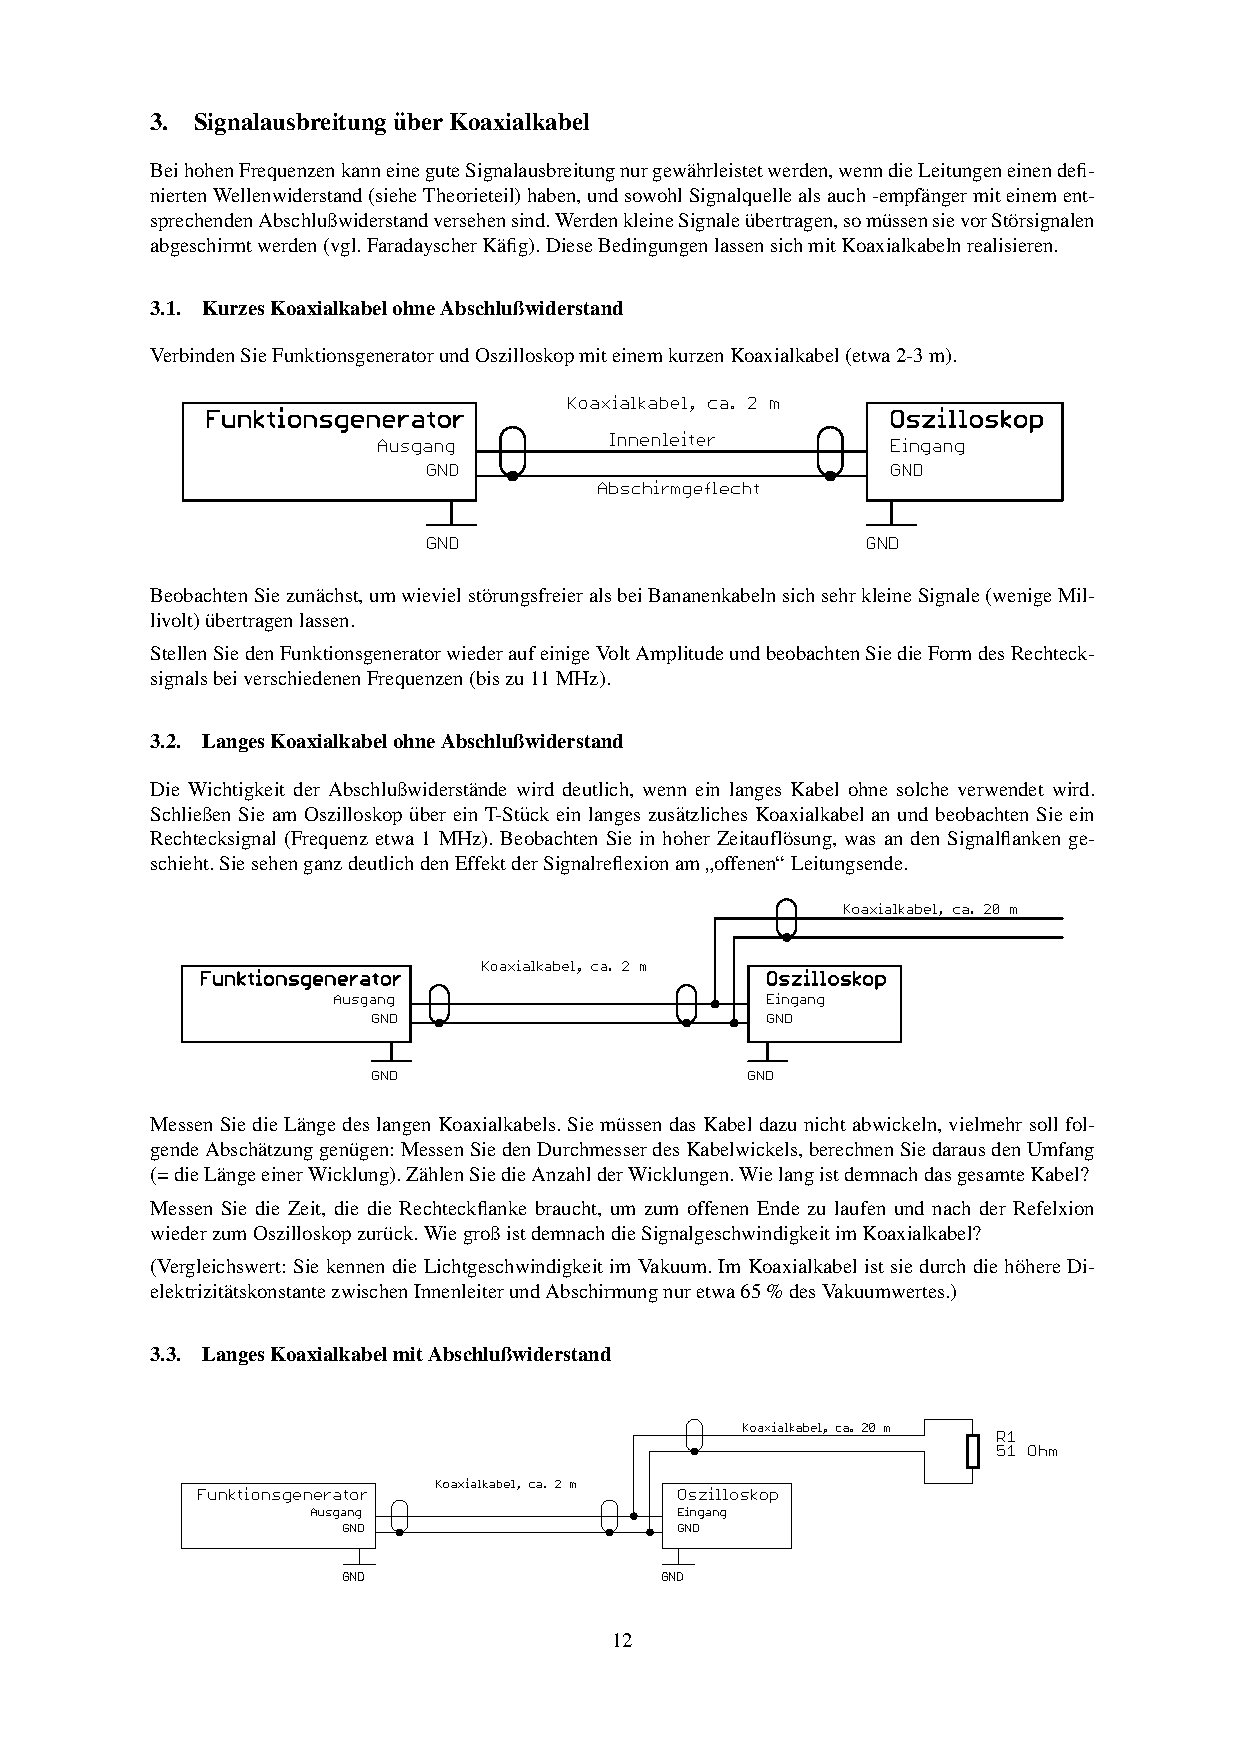
\includegraphics[trim = 10mm 25mm 10mm 235mm, clip, scale = 1]{3-3_3.pdf}
  	\caption[Schaltskizze einer Verbindung zwischen Funktionsgenerator und Oszilloskop, mit langem Koaxialkabel und Abschlusskabel]{Schaltskizze einer Verbindung zwischen Funktionsgenerator und Oszilloskop, mit langem Koaxialkabel und Abschlusskabel\footnotemark}
  \label{fig:3.3}
\end{figure}
\footnotetext{Abbildung entnommen von http://www.atlas.uni-wuppertal.de/$\sim$kind/ep1\_14.pdf Seite 12 am 19.10.2014}


\begin{figure}[H] 
  \centering
    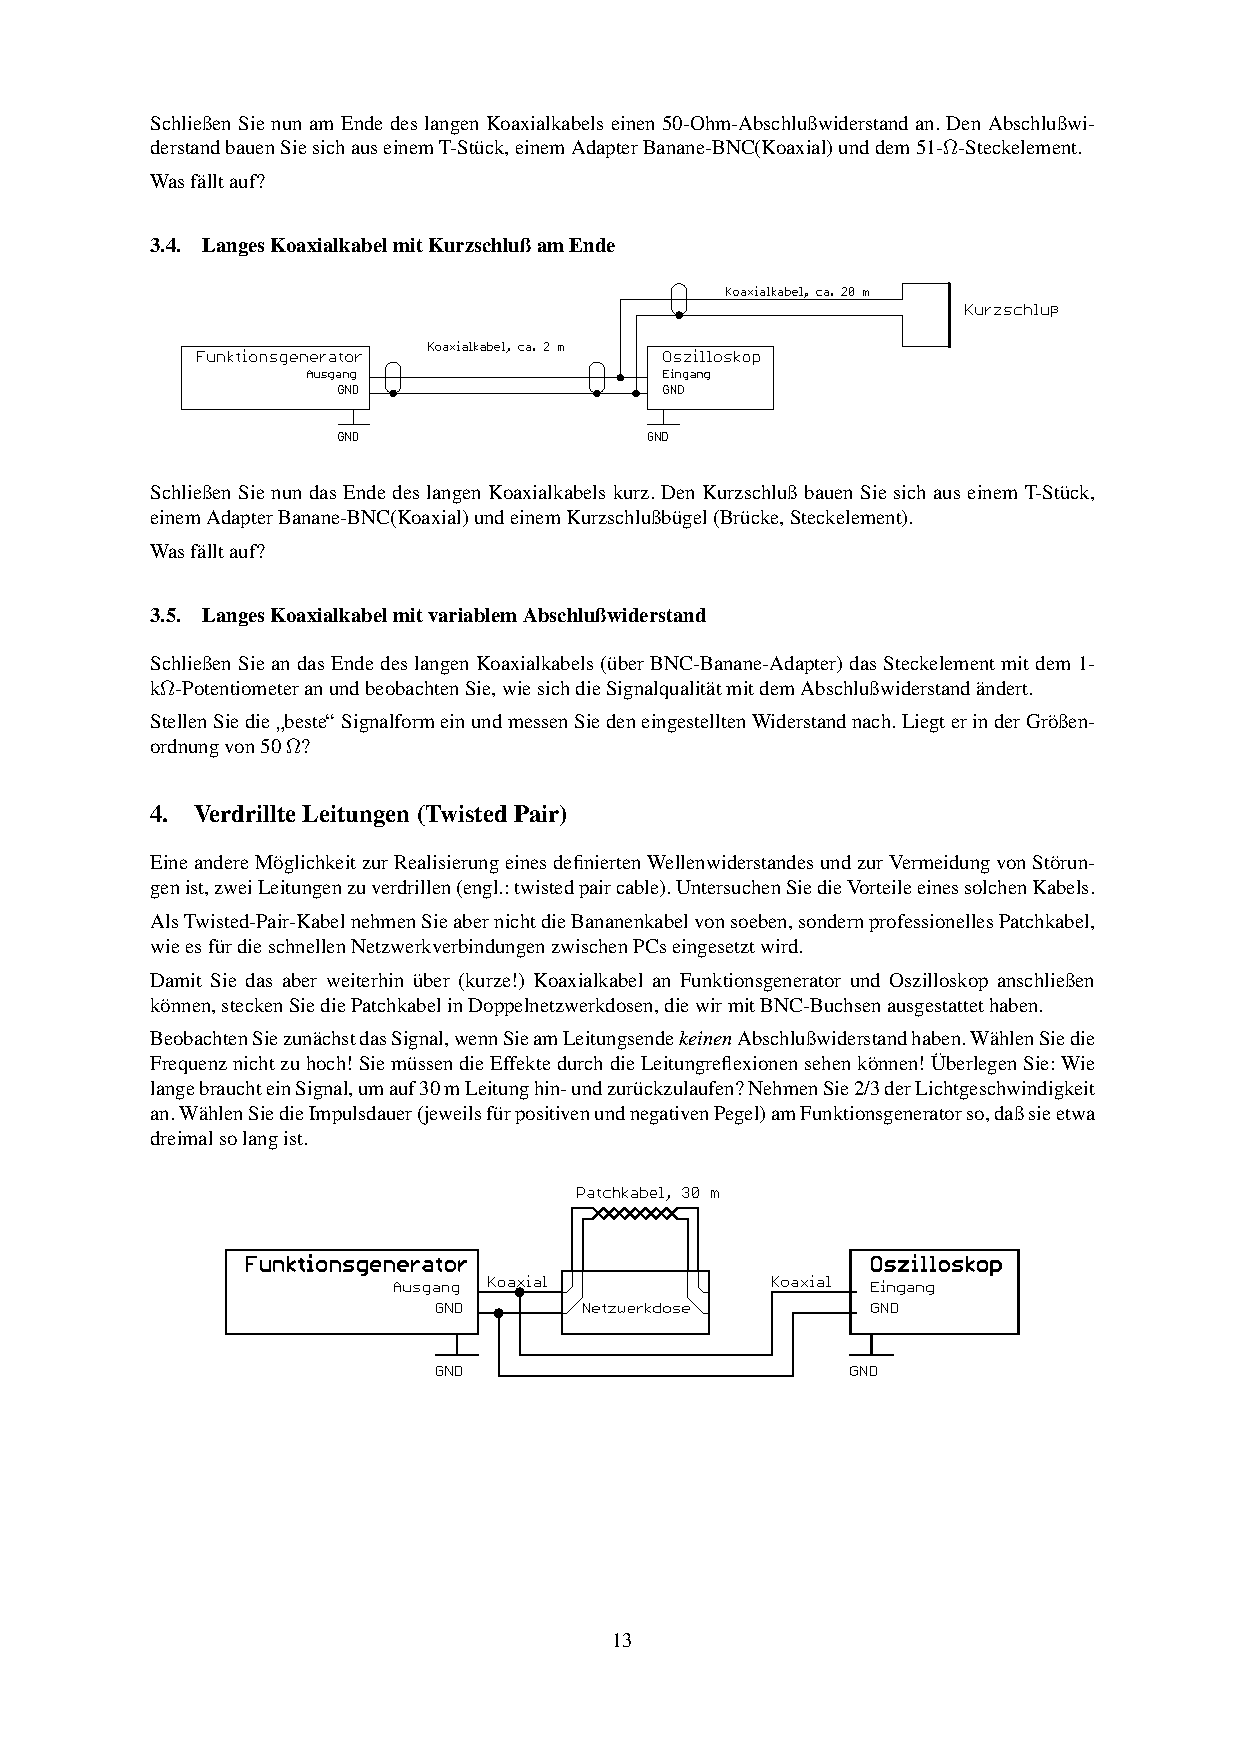
\includegraphics[trim = 10mm 220mm 10mm 45mm, clip, scale = 1]{3_4-4.pdf}
  	\caption[Schaltskizze einer Verbindung zwischen Funktionsgenerator und Oszilloskop, mit langem Koaxialkabel und Kurzschluss]{Schaltskizze einer Verbindung zwischen Funktionsgenerator und Oszilloskop, mit langem Koaxialkabel und Kurzschluss\footnotemark}
  \label{fig:3.4}
\end{figure}
\footnotetext{Abbildung entnommen von http://www.atlas.uni-wuppertal.de/$\sim$kind/ep1\_14.pdf Seite 13 am 19.10.2014}


\begin{figure}[H] 
  \centering
    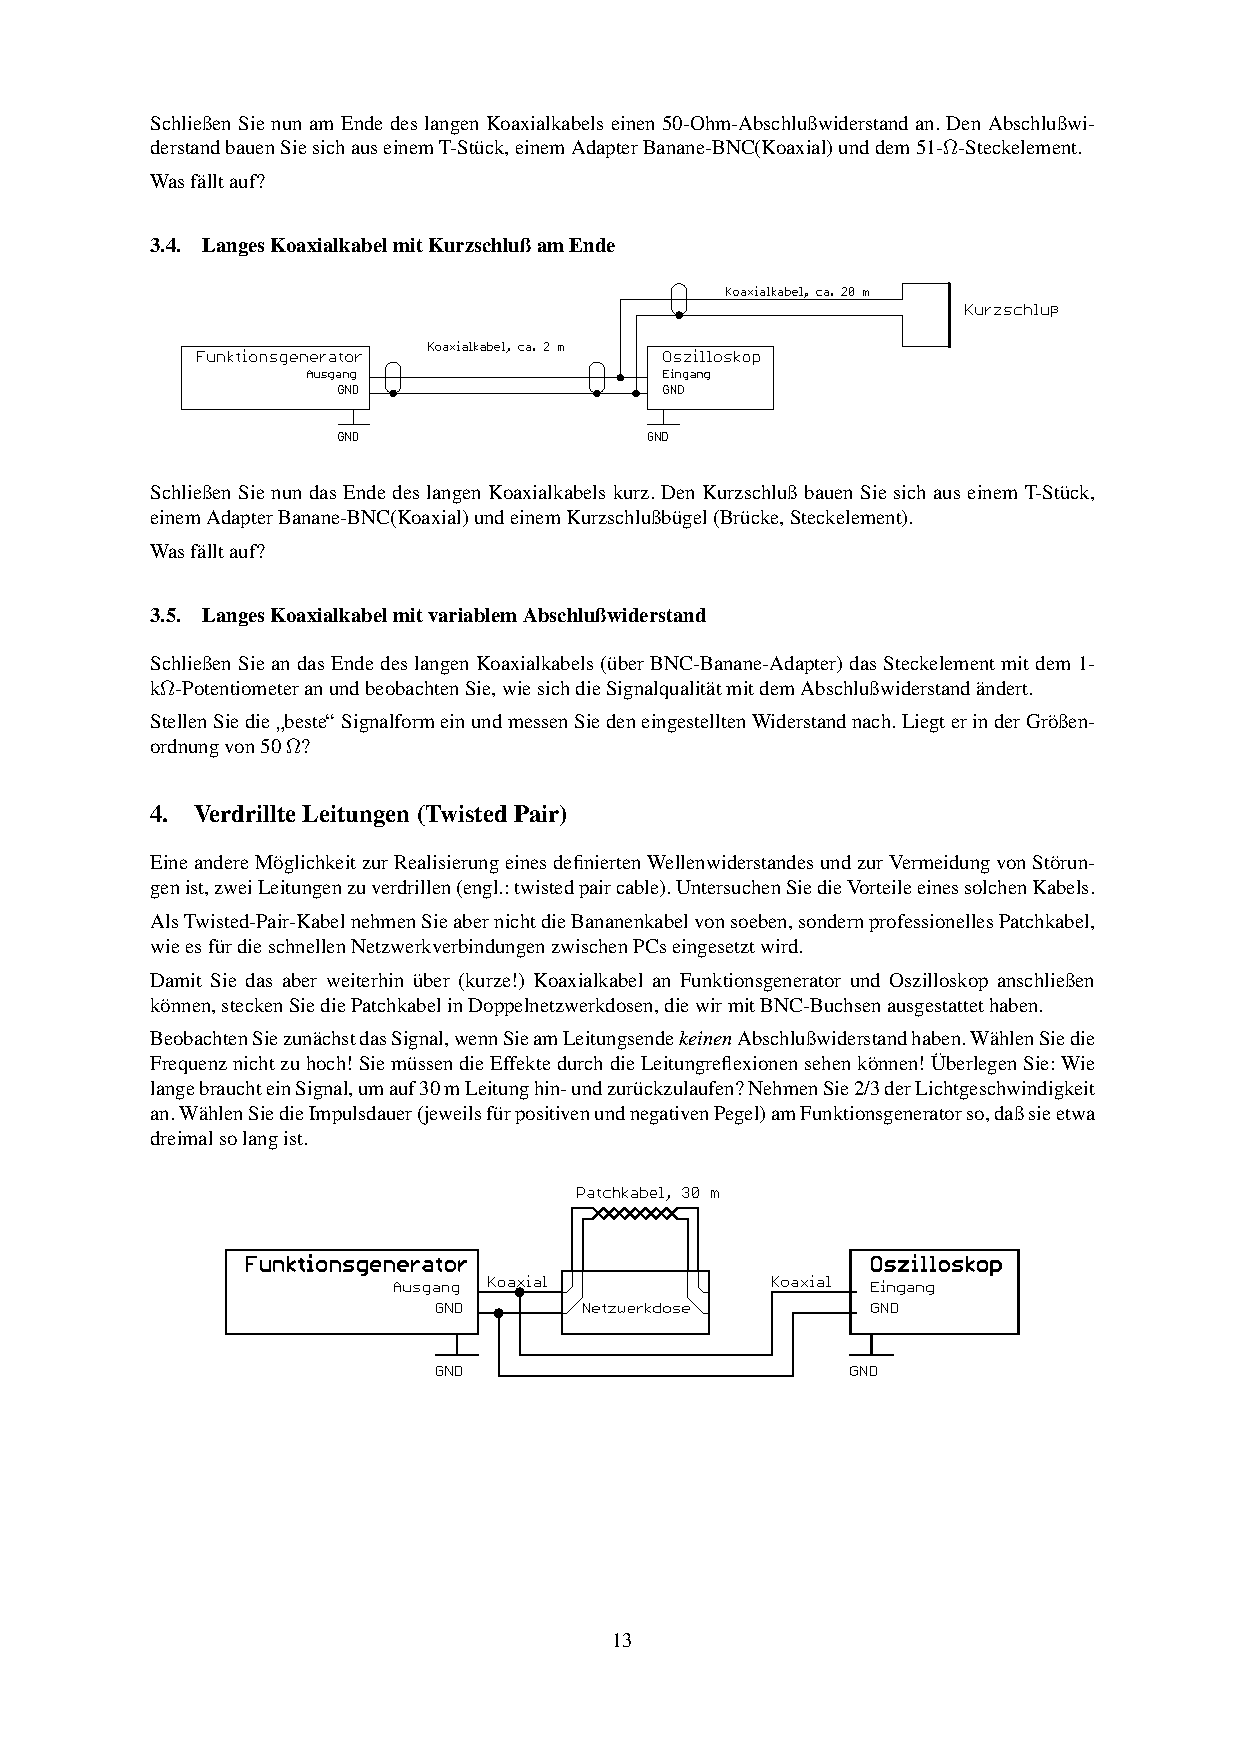
\includegraphics[trim = 10mm 60mm 10mm 200mm, clip, scale = 1]{3_4-4.pdf}
  	\caption[Schaltskizze einer Verbindung zwischen Funktionsgenerator und Oszilloskop, mit Patch- und Koaxialkabel]{Schaltskizze einer Verbindung zwischen Funktionsgenerator und Oszilloskop, mit Patch- und Koaxialkabel\footnotemark}
  \label{fig:4.1}
\end{figure}
\footnotetext{Abbildung entnommen von http://www.atlas.uni-wuppertal.de/$\sim$kind/ep1\_14.pdf Seite 14 am 19.10.2014}


\begin{figure}[H] 
  \centering
    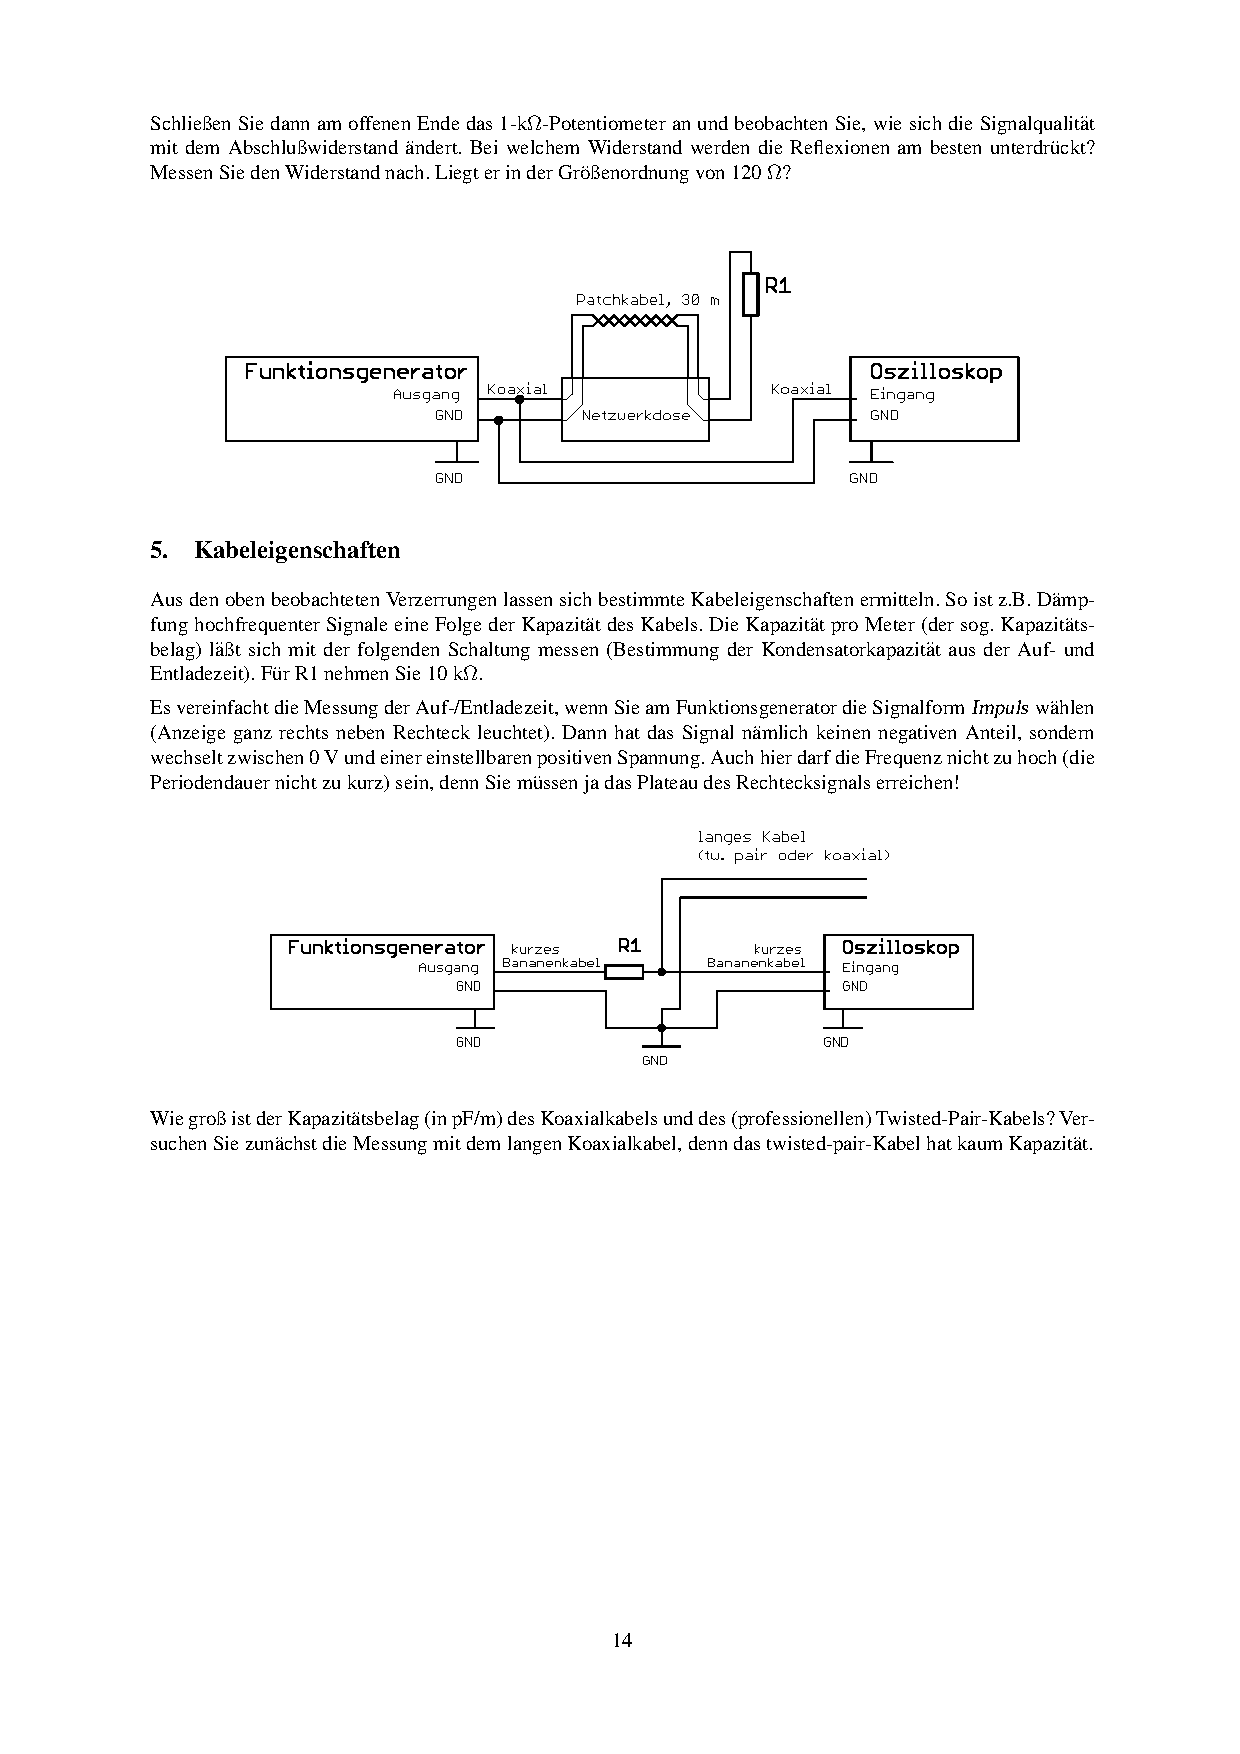
\includegraphics[trim = 10mm 210mm 10mm 40mm, clip, scale = 1]{4-5.pdf}
  	\caption[Schaltskizze einer Verbindung zwischen Funktionsgenerator und Oszilloskop, mit Patch- und Koaxialkabel (geschlossen mit Potentiometer)]{Schaltskizze einer Verbindung zwischen Funktionsgenerator und Oszilloskop, mit Patch- und Koaxialkabel (geschlossen mit Potentiometer)\footnotemark}
  \label{fig:4.2}
\end{figure}
\footnotetext{Abbildung entnommen von http://www.atlas.uni-wuppertal.de/$\sim$kind/ep1\_14.pdf Seite 14 am 19.10.2014}


\begin{figure}[H] 
  \centering
    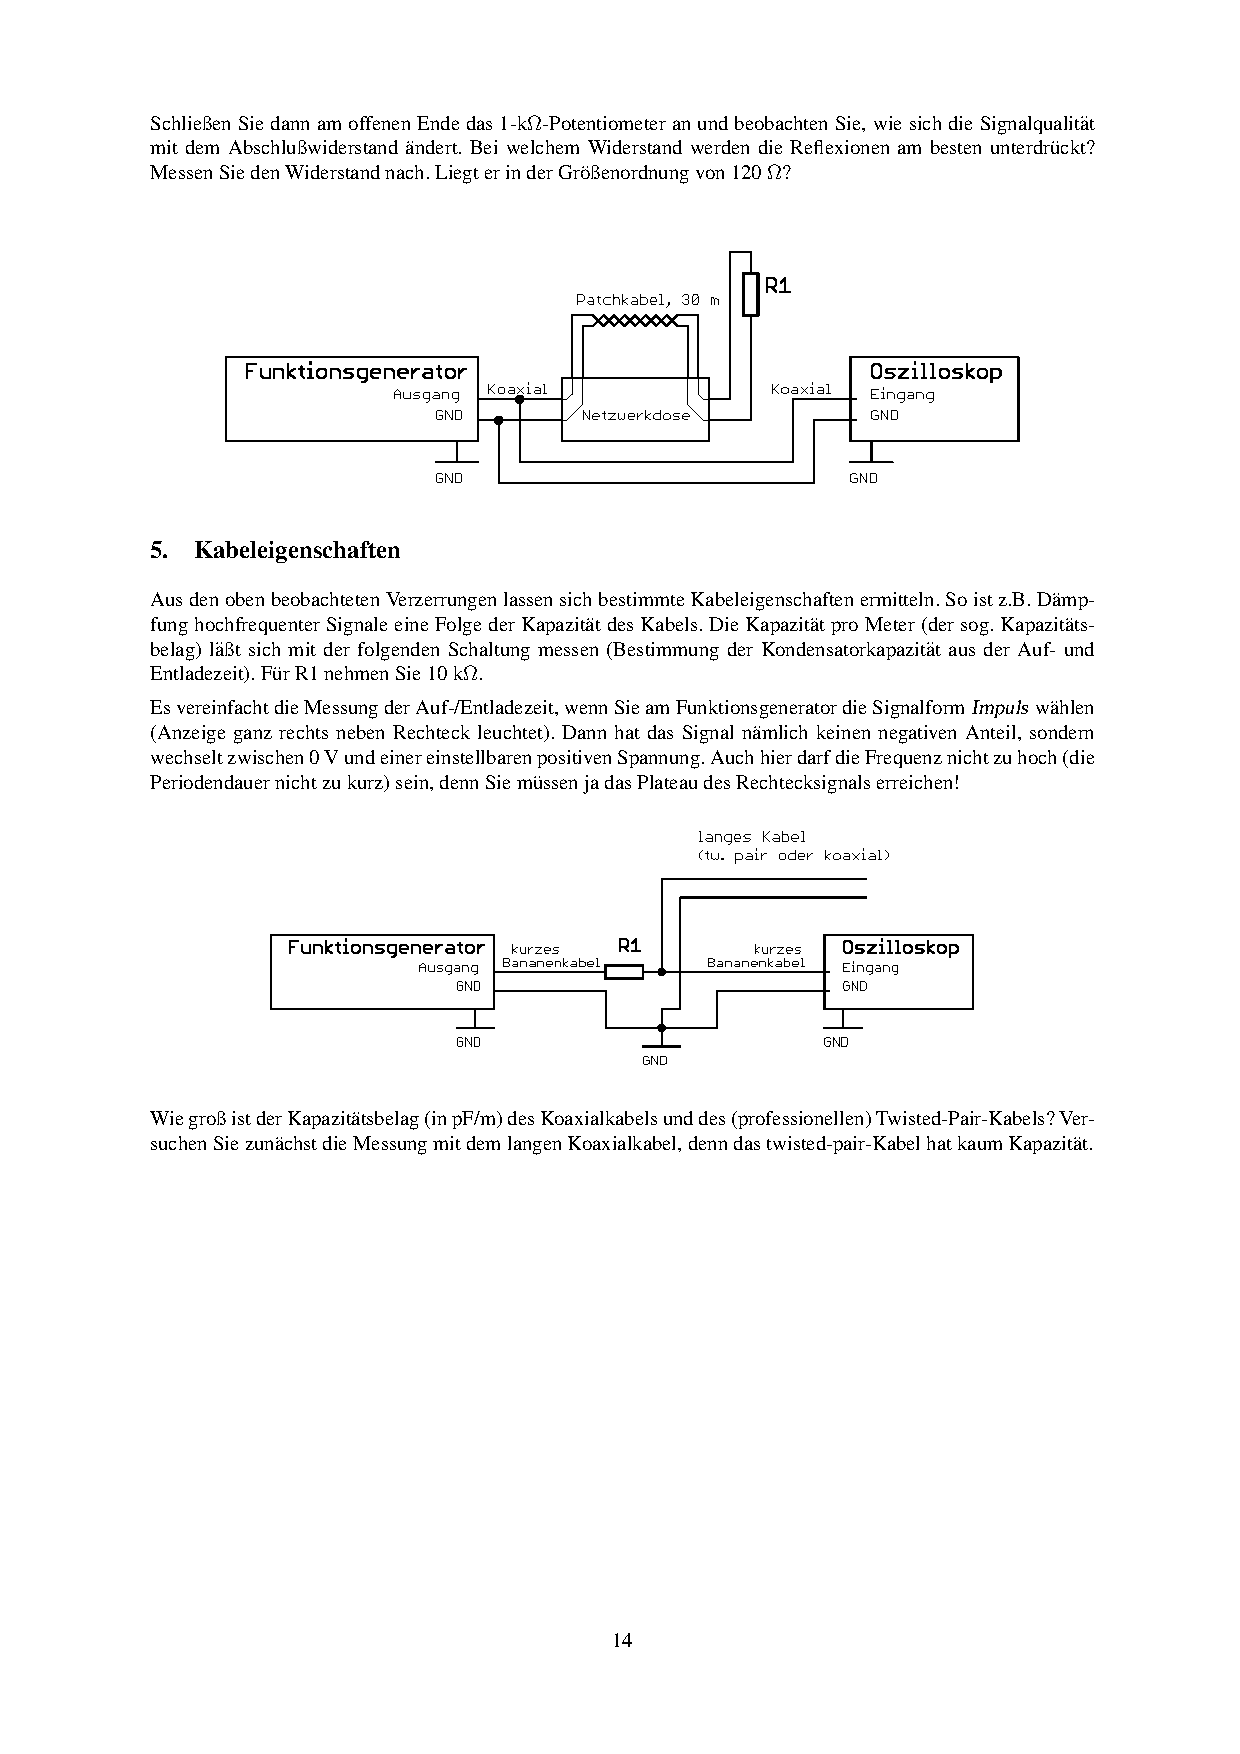
\includegraphics[trim = 10mm 110mm 10mm 140mm, clip, scale = 1]{4-5.pdf}
  	\caption[Schaltskizze zur Bestimmung des Kapazitätsbelags]{Schaltskizze zur Bestimmung des Kapazitätsbelags\footnotemark}
  \label{fig:5}
\end{figure}
\footnotetext{Abbildung entnommen von http://www.atlas.uni-wuppertal.de/$\sim$kind/ep1\_14.pdf Seite 14 am 19.10.2014}

\newpage\section{Einleitung}
%einleitung zu dem experiment.
%auf die einstellungen, die vor dem versuch gemacht werden, eingehen oder auf eine anleitung dazu verweisen.
%---------------------------------------------------------------------------------------------
%hinter der einleitung kann der allgemeine theoretische hintergrund in einer zusätzlichen section erklärt werden
Dieser Versuch beschäftigt sich mit den Übertragungseigenschaften verschiedener Kabel. Untersucht werden Bananenkabel, BNC-Kabel und Patchkabel.\newline
In den Aufbauten wird die Signalqualität der Kabel abhängig von der Einstellung des Funktionsgenerators (Sinus oder Rechteck), der Kabellänge und der Schaltung miteinder verglichen.\newline
Der sogenannte 'Kapazitätsbelag' (Kapazität zwischen Signal und Masseleitung) des BNC- und Patchkabels, welcher neben drei weiteren Kabelkonstanten (Selbstinduktivität der Leitung, Widerstand der Signalleitung, Leitwert der Isolation) bei der Beschreibung der Kabeleigenschaften eine wichtige Rolle spielt wird ebenfalls bestimmt.

\section{Verwendete Materialien}
%(immer) eine skizze oder ein foto einfügen, die geräte/materialien !nummerieren! und z.b. eine legende dazu schreiben
%falls am anfang des versuches nicht klar ist, was alles verwendet wird, wenn möglich erst am ende ein großes foto von den verwendeten materialien machen!
%-------------------------------------------------------------------------------------------
%ab hier für jeden versuchsteil einzeln, falls noch materialien hinzugenommen wurden immer im versuchsaufbau erwähnen!
\section{Versuchsteil...}
%kurz das ziel dieses versuchsteiles ansprechen, damit keine zwei überschriften direkt übereinander stehen!
%bei schwierigeren versuchen kann auch der theoretische hintergrund erläutert werden. (mit formeln, herleitungen und erklärungen)
\subsection{Versuchsaufbau}
%skizze zum versuchsaufbau (oder foto) einfügen,   es muss erklärt werden wie das ganze funktioniert und welche speziellen einstellungen verwendet wurden (z.b. welche knöpfe an den geräten für die messung verdreht wurden)
\subsection{Versuchsdurchführung}
%erklären, !was! wir machen, !warum! wir das machen und mit welchem ziel
%(wichtig) präzize erklären, wie bei dem versuch vorgegangen und was gemacht wurde
\subsection{Verwendete Formeln}
%eine legende kann angefertigt werden, die selbstverständlichen buchstaben müssen nicht extra erklärt werden
%mit knappen erklärungen die !verwendeten! formeln, sowie die zugehörige fehlerrechnung einfügen.
\subsection{Messergebnisse}
%die messwerte in !übersichtlichen! tabellen angegeben
%zu viele kleine tabellen in große tabellen überführen!
%zu große tabellen mit dem [scale]-befehl scalieren oder (falls zu lang) in zwei kleinere tabellen aufteilen
%(wichtig) vor !jeder! tabelle sagen, was gemessen wurde und wie die fehler gewählt wurden und ausreichend !erklären!, !warum! wir unsere fehler grade so gewählt haben
\subsection{Auswertung}
%zuerst !alle! errechneten werte entweder in ganzen sätzen aufzählen, oder in tabellen (übersichtlicher) dargestellen, sowie auf die verwendeten formeln verweisen (die referenzierung der formel kann in der überschrift stehen)
%kurz erwähnen (vor der tabelle), warum wir das ganze ausrechnen bzw. was wir dort ausrechnen
%danach histogramme und plots erstellen, wobei wenn möglich funktionen durch die plots gelegt werden (zur not können auch splines benutzt werden, was aber angegeben werden muss)
%bei fits immer die funktion und das reduzierte chiquadrat mit angegeben, wobei auf verständlichkeit beim entziffern der zehnerpotenzen geachtet werden muss z.b. f(x)=(wert+-fehler)\cdot10^{irgendeine zahl}\cdot x + (wert+-fehler)\cdot10^{irgendeine zahl}
%bei jedem fit erklären, nach welchem zusammenhang gefittet wurde und warum!
%bei plots darauf achten, dass die achsenbeschriftung (auch die tics) die richtige größe haben und die legende im plot nicht die messwerte verdeckt
%kurz die aufgabenstellung abgehandeln
\subsection{Diskussion}
%(immer) die gemessenen werte und die bestimmten werte über die messfehler mit literaturwerten oder untereinander vergleichen
%in welchem fehlerintervall des messwertes liegt der literaturwert oder der vergleichswert?
%wie ist der relative anteil des fehlers am messwert und damit die qualität unserer messung?
%in einem satz erklären, wie gut unser fehler und damit unsere messung ist
%kurz erläutern, wie systematische fehler unsere messung beeinflusst haben könnten
%(wichtig) zum schluss ansprechen, in wie weit die ergebnisse mit der theoretischen vorhersage übereinstimmen
%--------------------------------------------------------------------------------------------
%falls tabellen mit den messwerten zu lang werden, kann die section mit den messwerten auch hinter der diskussion angefügt bzw. eine section mit dem anhang eingefügt werden.





\section{Signalausbreitung über einfache Kabel}
%kurz das ziel dieses versuchsteiles ansprechen, damit keine zwei überschriften direkt übereinander stehen!
%bei schwierigeren versuchen kann auch der theoretische hintergrund erläutert werden. (mit formeln, herleitungen und erklärungen)
Im zweitem Versuchsteil sollte die Störanfälligkeit von Signalen bei Übertragung mit Bananenkabeln überprüft werden. Dabei wurden drei verschiedene Übertragungsmöglichkeiten verwendet, Übertragung mit nur einem Bananenkabel, mit zwei Bananenkabeln und mit einem twisted-pair Kabel aus zwei Bananenkabeln.
\subsection{Versuchsaufbau}
%skizze zum versuchsaufbau (oder foto) einfügen,   es muss erklärt werden wie das ganze funktioniert und welche speziellen einstellungen verwendet wurden (z.b. welche knöpfe an den geräten für die messung verdreht wurden)

Der Versuchsaufbau teilt sich in drei Teile auf.

\subsubsection{Versuchsteil 2.1}

Für die Signalübertragung mit nur einem Bananenkabel wurde der Aufbau aus Abbildung \ref{fig:2.1} verwendet.

\begin{figure}[H] 
  \centering
    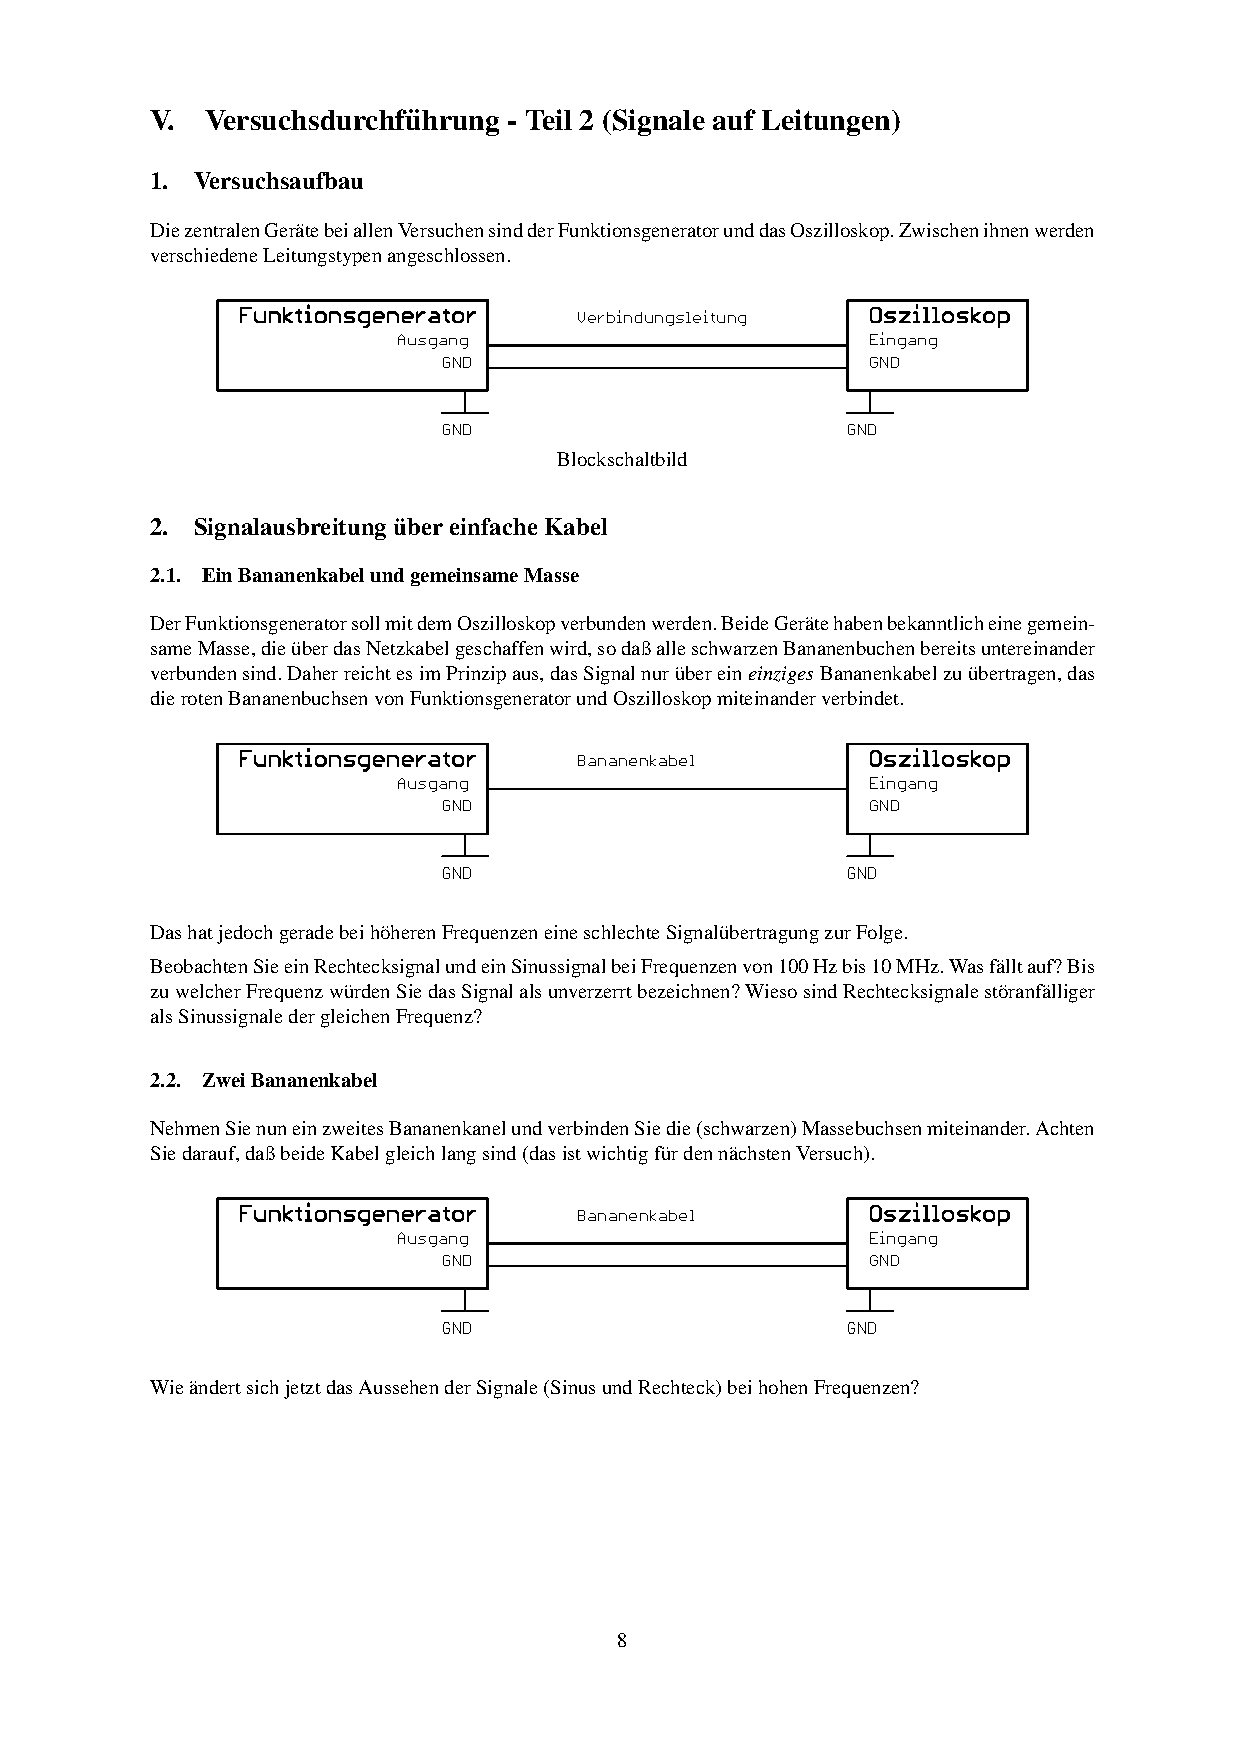
\includegraphics[trim = 10mm 142mm 10mm 125mm, clip, scale = 1]{2_0-2_2.pdf}
  	\caption[Schaltskizze einer Verbindung zwischen Funktionsgenerator und Oszilloskop, mit einem Bananenkabel]{Schaltskizze einer Verbindung zwischen Funktionsgenerator und Oszilloskop, mit einem Bananenkabel\footnotemark}
  \label{fig:2.1}
\end{figure}
\footnotetext{Abbildung entnommen von http://www.atlas.uni-wuppertal.de/$\sim$kind/ep1\_14.pdf Seite 8 am 19.10.2014}

\subsubsection{Versuchsteil 2.2}

Bei der Signalübertragung mit zwei Bananenkabeln wurde der Aufbau von Abbildung \ref{fig:2.1} verwendet.

\begin{figure}[H] 
  \centering
    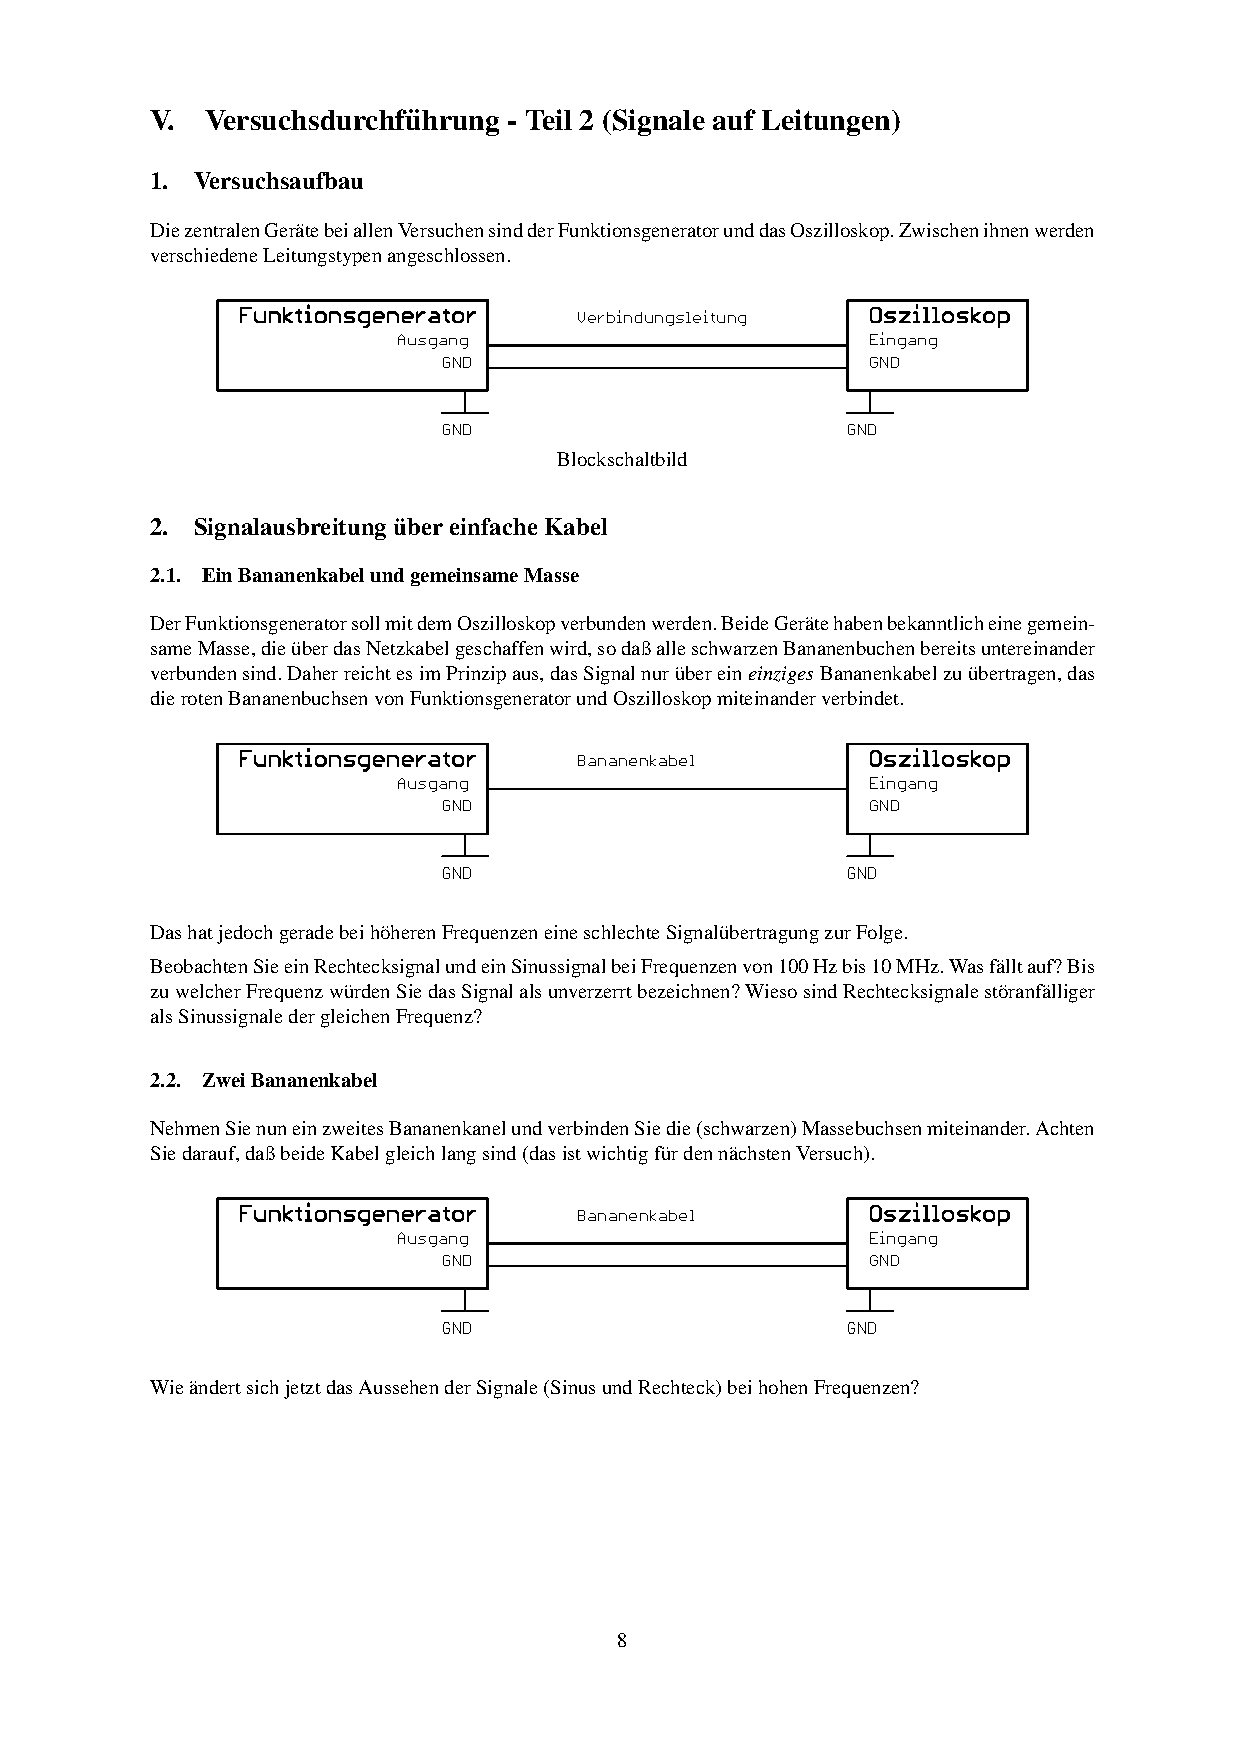
\includegraphics[trim = 10mm 70mm 10mm 200mm, clip, scale = 1]{2_0-2_2.pdf}
  	\caption[Schaltskizze einer Verbindung zwischen Funktionsgenerator und Oszilloskop, mit zwei Bananenkabeln]{Schaltskizze einer Verbindung zwischen Funktionsgenerator und Oszilloskop, mit zwei Bananenkabeln\footnotemark}
  \label{fig:2.2}
\end{figure}
\footnotetext{Abbildung entnommen von http://www.atlas.uni-wuppertal.de/$\sim$kind/ep1\_14.pdf Seite 8 am 19.10.2014}

\subsubsection{Versuchteil 2.3}

Für die Signalübertragung über ein twisted-pair Kabel wurden die Bananenkabel aus Abbildung \ref{fig:2.2} verdrillt.

\begin{figure}[H] 
  \centering
    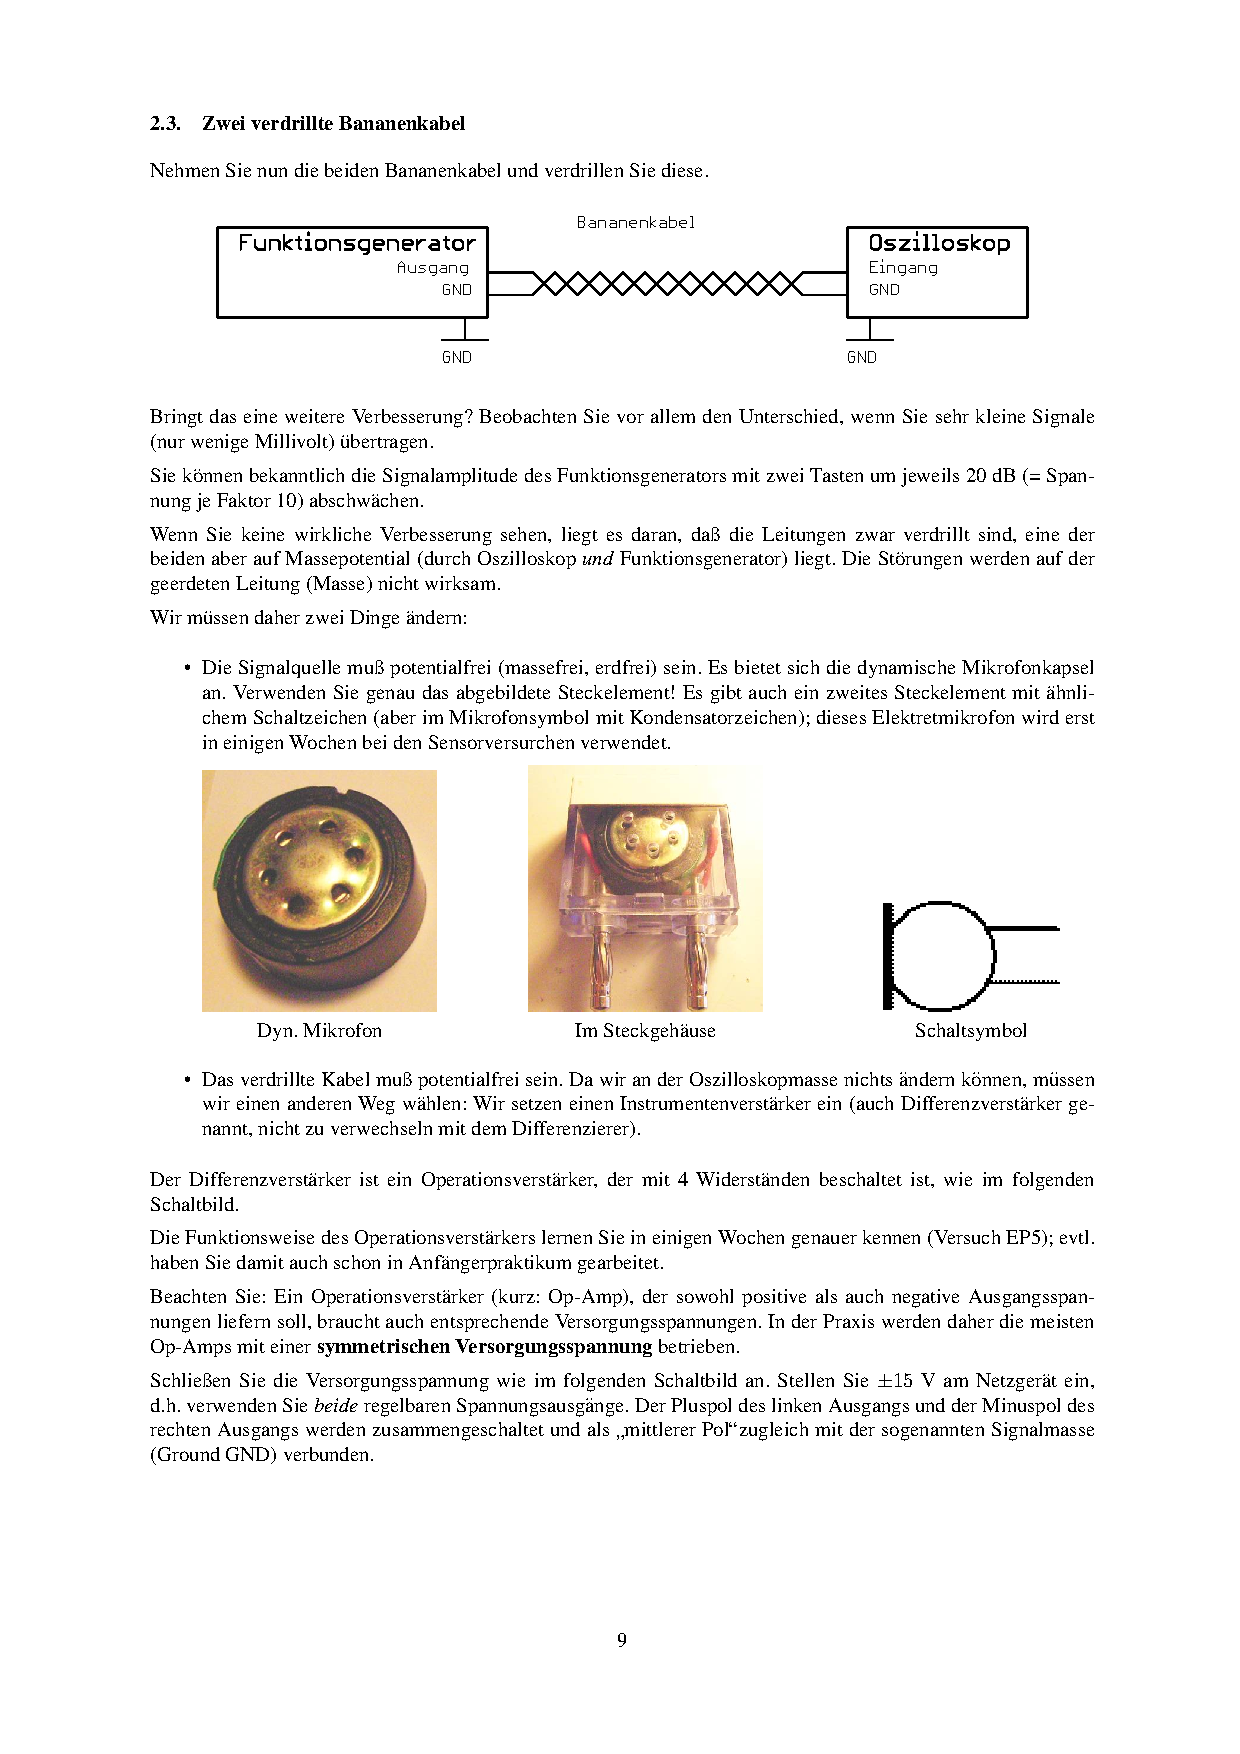
\includegraphics[trim = 10mm 230mm 10mm 32mm, clip, scale = 1]{2_3.pdf}
  	\caption[Schaltskizze einer Verbindung zwischen Funktionsgenerator und Oszilloskop, mit zwei verdrillten Bananenkabeln]{Schaltskizze einer Verbindung zwischen Funktionsgenerator und Oszilloskop, mit zwei verdrillten Bananenkabeln\footnotemark}
  \label{fig:2.3}
\end{figure}
\footnotetext{Abbildung entnommen von http://www.atlas.uni-wuppertal.de/$\sim$kind/ep1\_14.pdf Seite 9 am 19.10.2014}

Als alternative zu dem geerdetem Funktionsgenerator wird ein Mikrofon als Signalquelle verwendet. Das Signal wir über einen Operationsverstärker, siehe Abbildung \ref{fig:2.33} verstärkt, um das Signal auf dem Oszilloskop sichtbar zu machen.

\begin{figure}[H] 
  \centering
    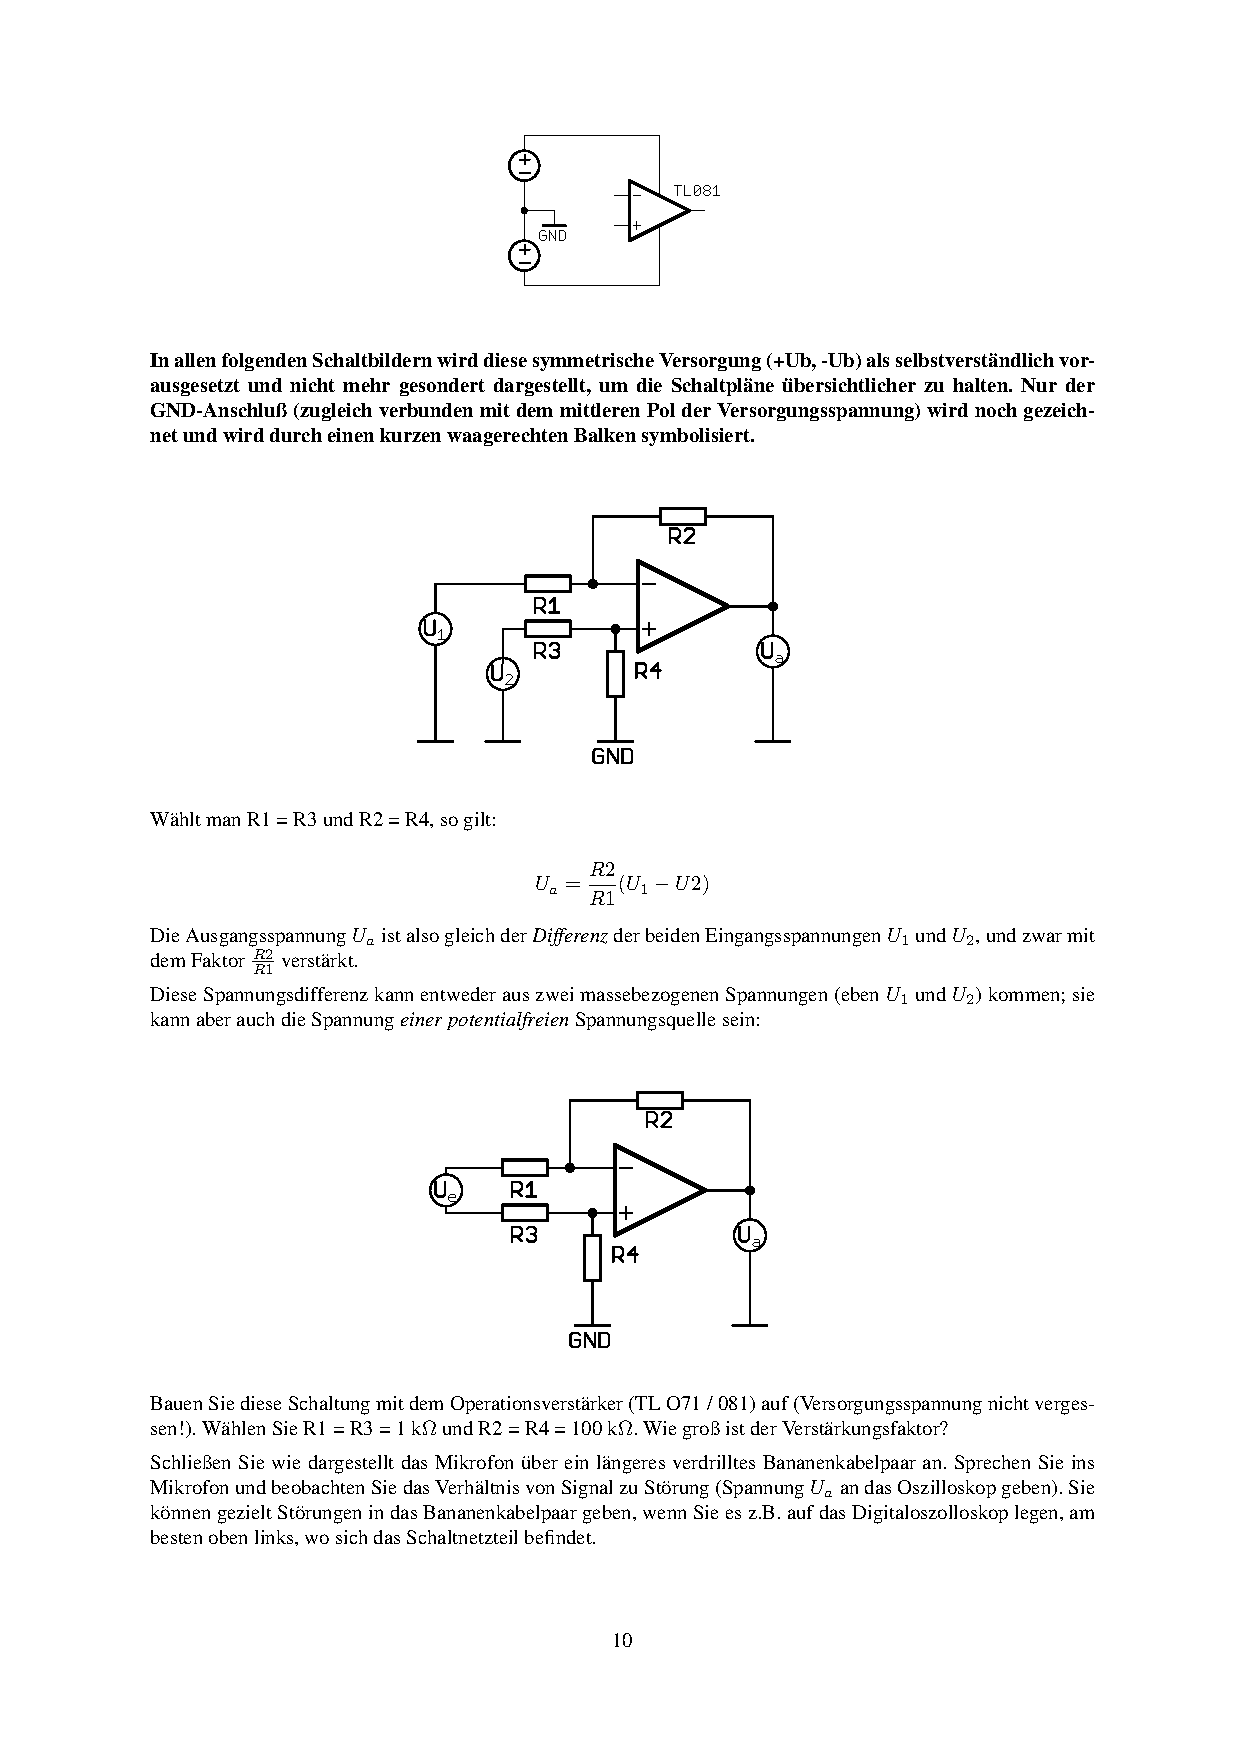
\includegraphics[trim = 10mm 240mm 10mm 15mm, clip, scale = 1]{Op-Amp.pdf}
  	\caption[Schaltskizze zum Anschlusses des Operationsverstärkers]{Schaltskizze zum Anschlusses des Operationsverstärkers\footnotemark}
  \label{fig:2.33}
\end{figure}
\footnotetext{Abbildung entnommen von http://www.atlas.uni-wuppertal.de/$\sim$kind/ep1\_14.pdf Seite 11 am 19.10.2014}

Der Operationsverstärker und das Mikrofon werden dann nach Schaltbild \ref{fig:2.4} zusammen geschaltet.
Dabei wurde für die Widerstände die Werte R$_1$=R$_3$= 1k$\Omega$ und R$_2$=R$_4$=100k$\Omega$ gewählt, dadurch ergibt sich eine Verstärkung um den Faktor 100.

\begin{figure}[H] 
  \centering
    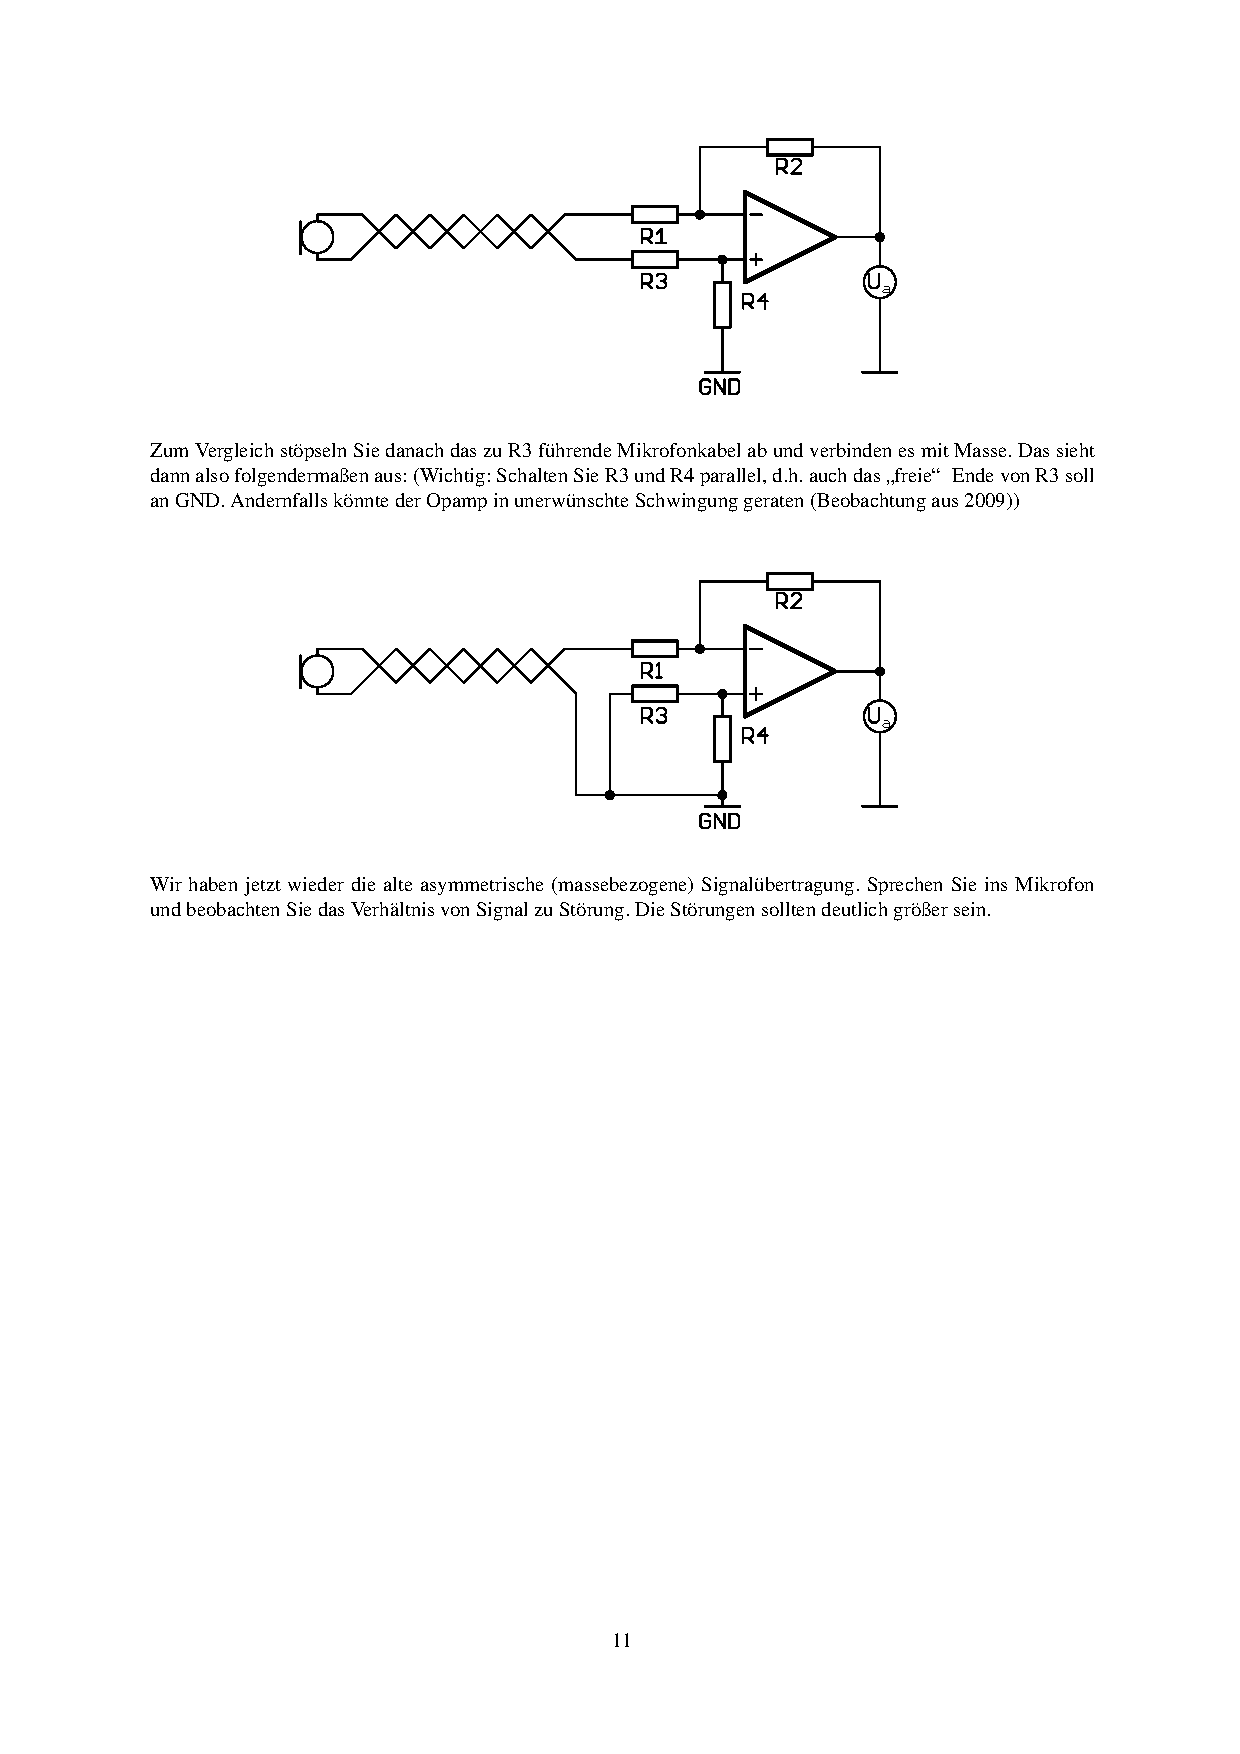
\includegraphics[trim = 10mm 230mm 10mm 20mm, clip, scale = 1]{2_3+Op-Amp.pdf}
  	\caption[Schaltskizze des Aufbaus mit Operationsverstärker und verdrillten Bananenkabeln]{Schaltskizze des Aufbaus mit Operationsverstärker und verdrillten Bananenkabeln\footnotemark}
  \label{fig:2.4}
\end{figure}
\footnotetext{Abbildung entnommen von http://www.atlas.uni-wuppertal.de/$\sim$kind/ep1\_14.pdf Seite 11 am 19.10.2014}

Zum Vergleich wird dann Widerstand 3 noch an die Massen angelegt, Aufbau nach Abbildung \ref{fig:2.5}.

\begin{figure}[H] 
  \centering
    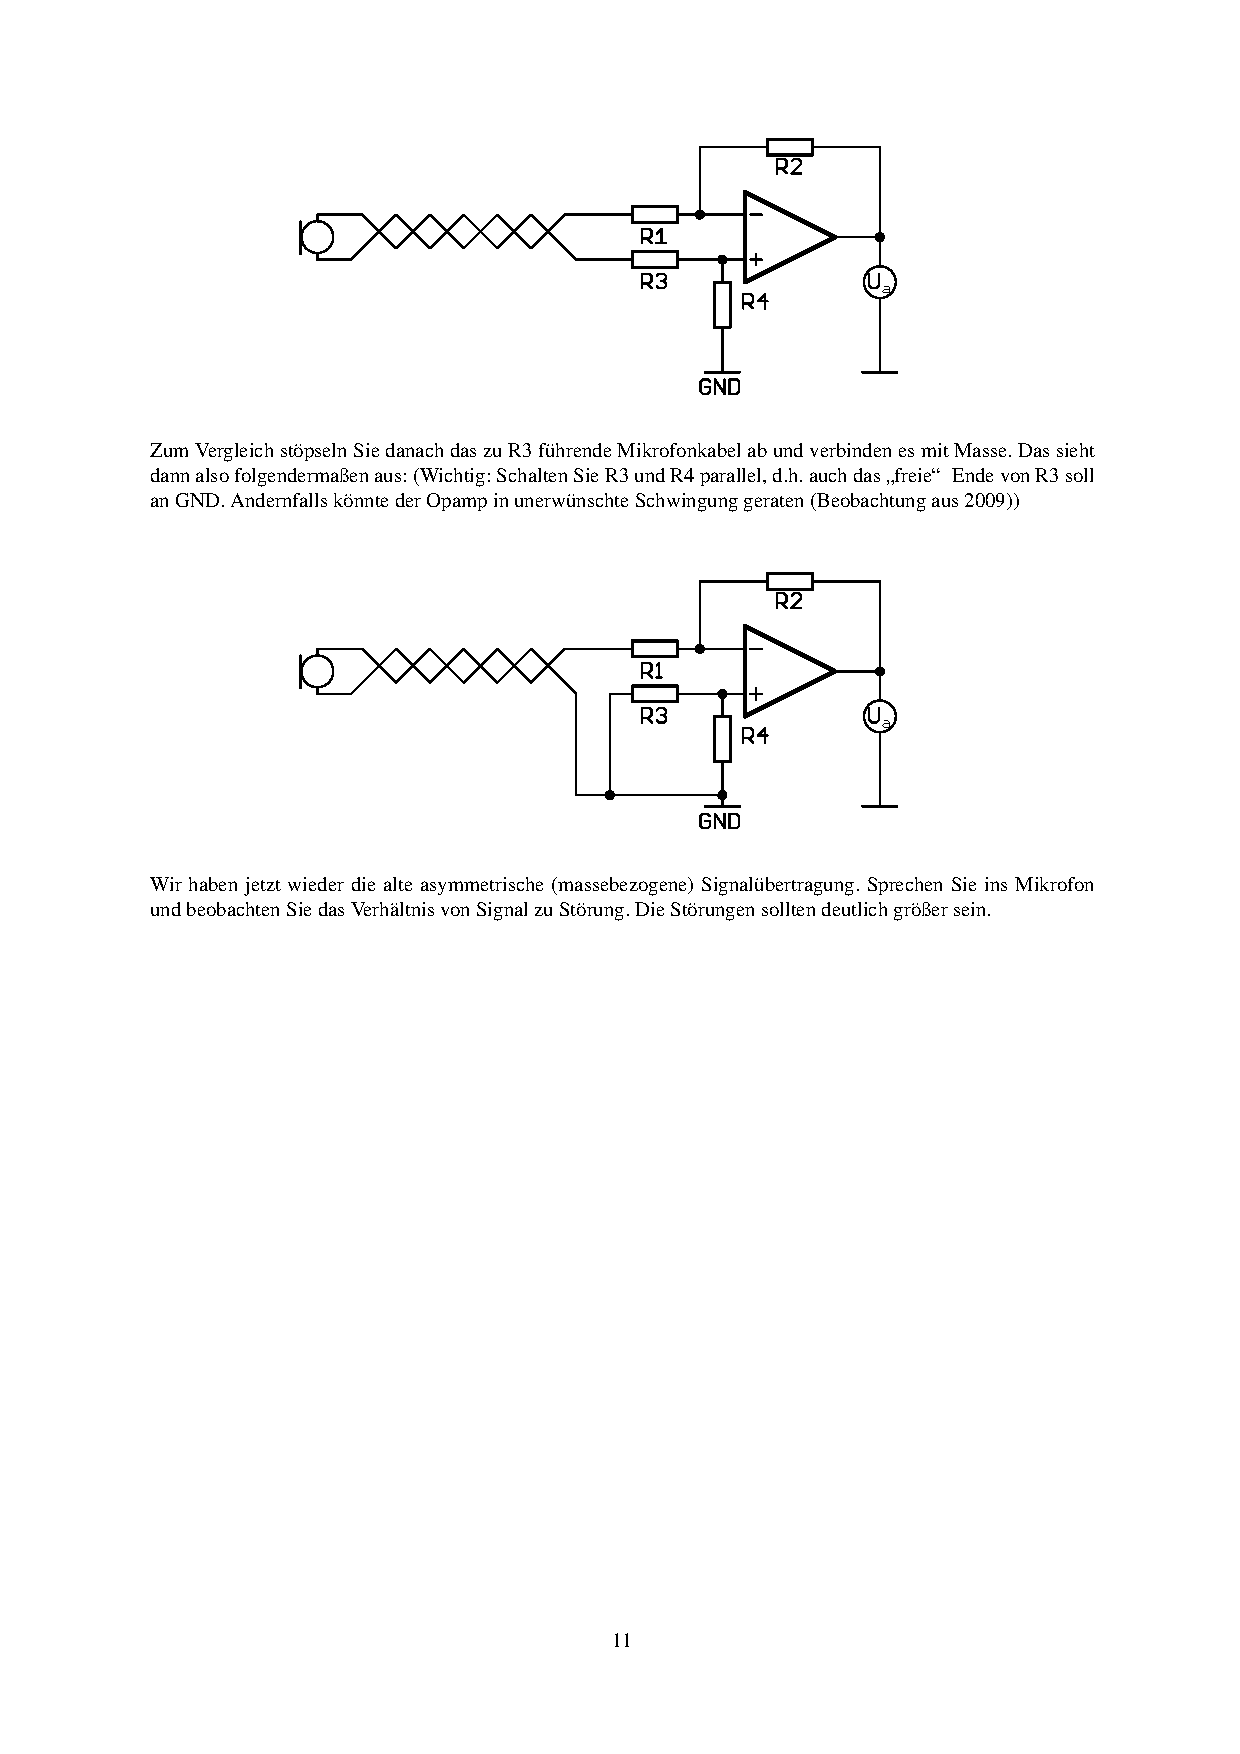
\includegraphics[trim = 10mm 160mm 10mm 90mm, clip, scale = 1]{2_3+Op-Amp.pdf}
  	\caption[Schaltskizze des Aufbaus mit Operationsverstärker und verdrillten Bananenkabeln, bei parallel geschaltetem R$_3$]{Schaltskizze des Aufbaus mit Operationsverstärker und verdrillten Bananenkabeln, bei parallel geschaltetem R$_3$\footnotemark}
  \label{fig:2.5}
\end{figure}
\footnotetext{Abbildung entnommen von http://www.atlas.uni-wuppertal.de/$\sim$kind/ep1\_14.pdf Seite 11 am 19.10.2014}


\subsection{Versuchsdurchführung}
%erklären, !was! wir machen, !warum! wir das machen und mit welchem ziel
%(wichtig) präzize erklären, wie bei dem versuch vorgegangen und was gemacht wurde
%erklären, !was! wir machen, !warum! wir das machen und mit welchem ziel
%(wichtig) präzize erklären, wie bei dem versuch vorgegangen und was gemacht wurde
An die Aufbauten in Versuchsteil 2.1 und 2.2 wurden jeweils eine Sinus- und eine Rechteckspannung angelegt und der Frequenzbereich von \unit[100]{Hz} bis \unit[10]{MHz} mit dem Oszilloskop ausgemessen. Die Verzerrungen des Signals werden anhand der Graphiken (bei gleichen Spannungsamplituden) miteinander verglichen.

Im dritten Teil werden die Bananenkabel aus dem zweiten Teil miteinander verdrillt und die Verbesserung der Signalübertragung bei kleinen Spannungsamplituden gegenüber dem Aufbau aus dem zweiten Teil verglichen.\newline
Da die Erdung des Funktionsgenerators und des Oszilloskops nur einen kleinen Gegenstrom durch das zweite Kabel zulässt, welcher eigentlich die Störung des zweiten Kabels aufheben soll, wird anschließend das Mikrofon als Signalquelle verwendet und über einen Operationsverstärker an das Oszilloskop angeschlossen, sodass durch das zweite Kabel der entgegengesetzte Strom fließen kann. Um die Verbesserung der Signalübertragung bei diesem Microphon (dynamisches Mikrophon) gegenüber dem geerdeten Fall abzuschätzen, wird parallel zu Widerstand R3 die Erde angeschlossen, sodass das zweite Kabel wie bei dem Aufbau mit dem Funktionsgenerator direkt mit der Erde verbunden ist. Für die Signalerzeugung wurde einerseits in das Mikrophon gepfiffen und andererseits das Mikrofon auf den Funktionsgenerator gelegt um die dadurch erzeugten Störsignale aufzunehmen. Die Darstellung wurde dann jeweils auf dem Oszilloskop angehalten.

%\subsection{Verwendete Formeln}
%eine legende kann angefertigt werden, die selbstverständlichen buchstaben müssen nicht extra erklärt werden
%mit knappen erklärungen die !verwendeten! formeln, sowie die zugehörige fehlerrechnung einfügen.

%\subsection{Messergebnisse}
%die messwerte in !übersichtlichen! tabellen angegeben
%zu viele kleine tabellen in große tabellen überführen!
%zu große tabellen mit dem [scale]-befehl scalieren oder (falls zu lang) in zwei kleinere tabellen aufteilen
%(wichtig) vor !jeder! tabelle sagen, was gemessen wurde und wie die fehler gewählt wurden und ausreichend !erklären!, !warum! wir unsere fehler grade so gewählt haben
\subsection{Auswertung}
%zuerst !alle! errechneten werte entweder in ganzen sätzen aufzählen, oder in tabellen (übersichtlicher) dargestellen, sowie auf die verwendeten formeln verweisen (die referenzierung der formel kann in der überschrift stehen)
%kurz erwähnen (vor der tabelle), warum wir das ganze ausrechnen bzw. was wir dort ausrechnen
%danach histogramme und plots erstellen, wobei wenn möglich funktionen durch die plots gelegt werden (zur not können auch splines benutzt werden, was aber angegeben werden muss)
%bei fits immer die funktion und das reduzierte chiquadrat mit angegeben, wobei auf verständlichkeit beim entziffern der zehnerpotenzen geachtet werden muss z.b. f(x)=(wert+-fehler)\cdot10^{irgendeine zahl}\cdot x + (wert+-fehler)\cdot10^{irgendeine zahl}
%bei jedem fit erklären, nach welchem zusammenhang gefittet wurde und warum!
%bei plots darauf achten, dass die achsenbeschriftung (auch die tics) die richtige größe haben und die legende im plot nicht die messwerte verdeckt
%kurz die aufgabenstellung abgehandeln

In der Auswertung wird die Qualität der übertragenen Signale bei unterschiedlichen Frequenzen überprüft.

\subsubsection{Versuchsteil 2.1}

Bei der ersten Messung mit nur einem Bananenkabel ergaben sich die folgenden Ergebnisse.
Bei der Übertragung des Sinussignals war kein qualitativer Unterschied fest zu stellen, wie man an Abbildung \ref{fig:2_1_sin_100hz} und Abbildung \ref{fig:2_1_sin_10mhz} erkennen kann.


\begin{figure}[H]
        \centering
        \begin{subfigure}[b]{0.48\textwidth}
                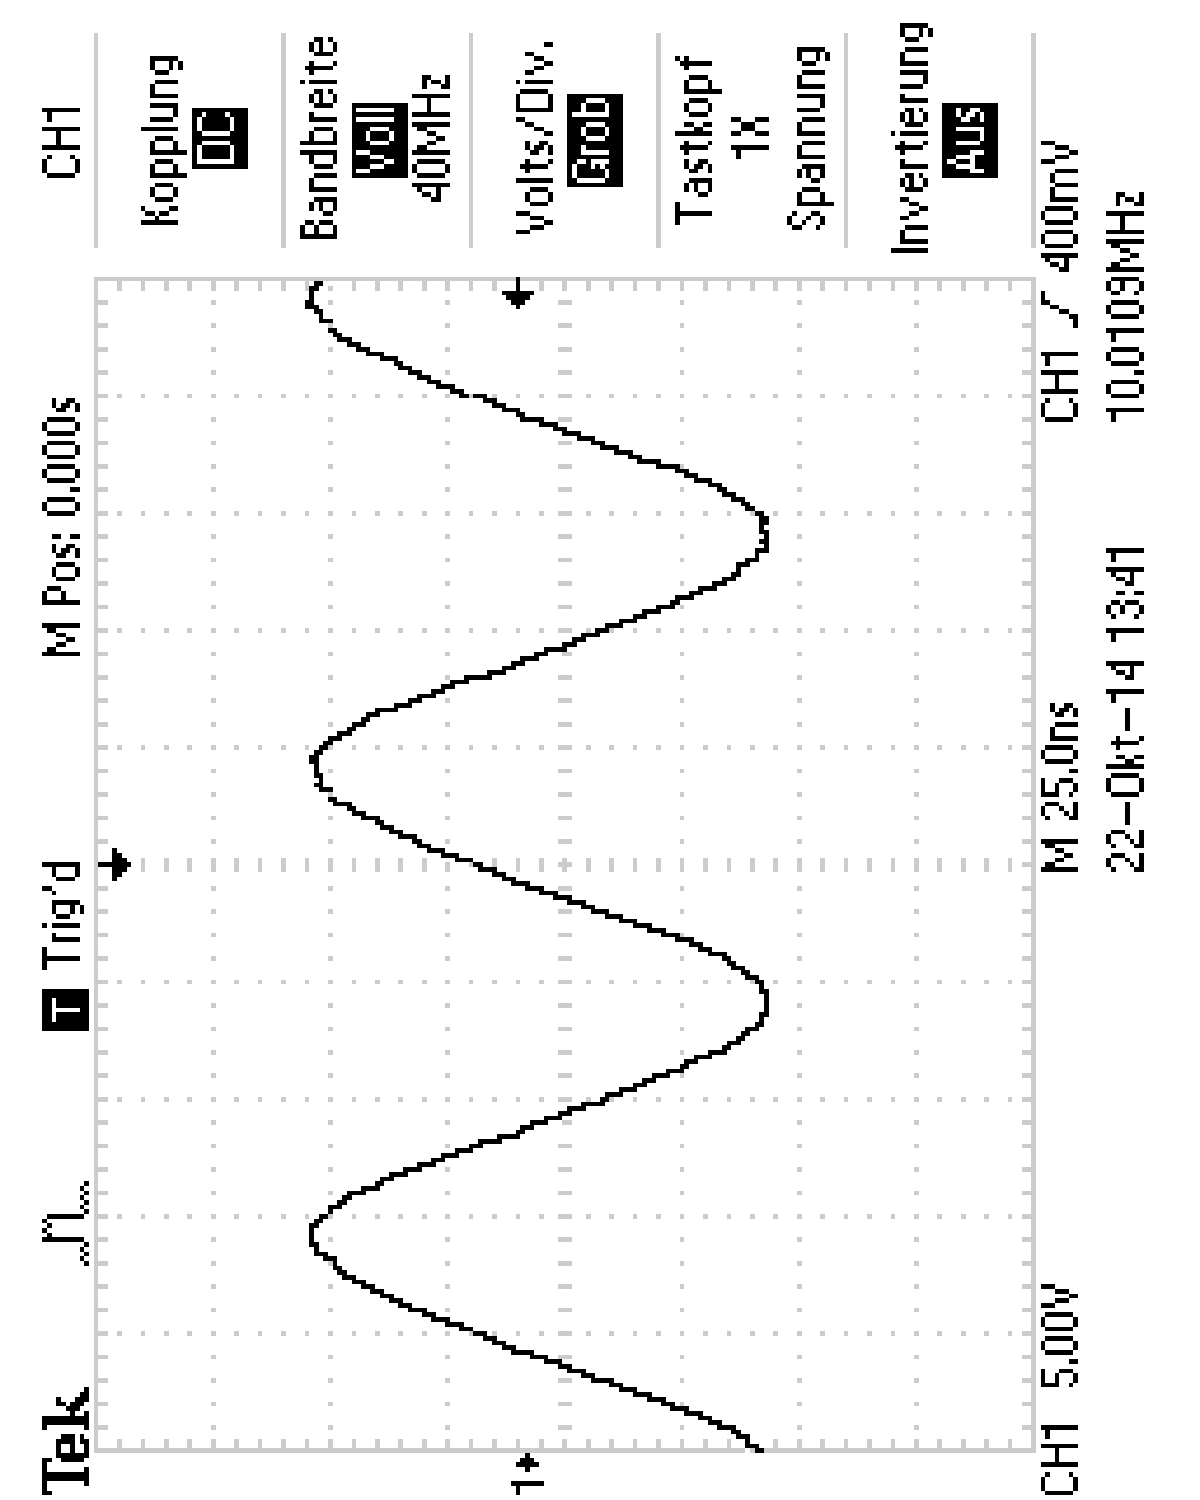
\includegraphics[width=\textwidth , scale = 0.4, angle = -90]{2_1_sin_10mhz.pdf}
                \caption[Aufnahme der Sinuswelle mit einer Frequenz von 100Hz]{Aufnahme der Sinuswelle mit einer Frequenz von 100Hz}
 				 \label{fig:2_1_sin_100hz}
        \end{subfigure}%
        ~ %add desired spacing between images, e. g. ~, \quad, \qquad, \hfill etc.
          %(or a blank line to force the subfigure onto a new line)
        \hfill
        \begin{subfigure}[b]{0.48\textwidth}
                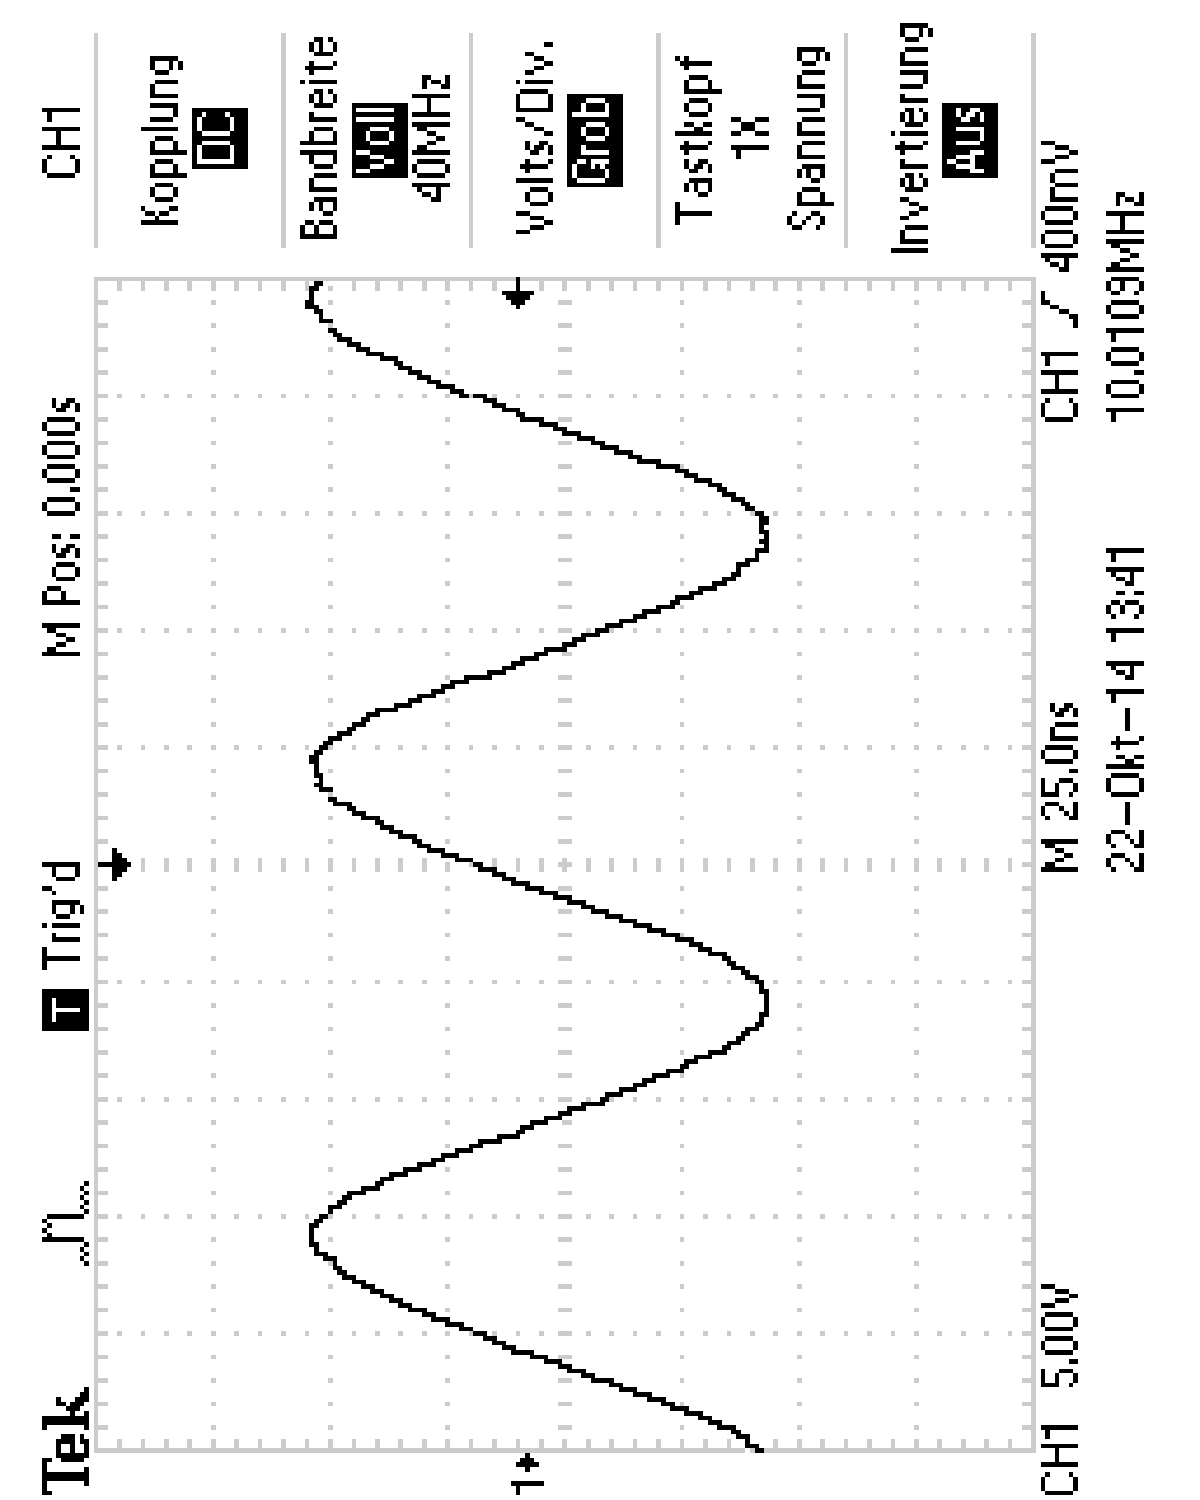
\includegraphics[width=\textwidth , scale = 0.4, angle = -90]{2_1_sin_10mhz.pdf}
                \caption[Aufnahme der Sinuswelle mit einer Frequenz von 10MHz]{Aufnahme der Sinuswelle mit einer Frequenz von 10MHz}
  				\label{fig:2_1_sin_10mhz}
        \end{subfigure}
        \caption{Kurve der übertragenen Sinussignale für 100Hz und 10MHz}
        \label{fig:2_1_sin_vergleich}
\end{figure}


Beim Messen des Signals der Rechteckspannung war bei 100Hz noch keine Verzerrung zu sehen, siehe Abbildung \ref{fig:2_1_rech_100hz}. Die ersten Verzerrungen wurden bei einer Frequenz von 10kHz gemessen, zu sehen in Abbildung \ref{fig:2_1_rech_10khz}. Bei einer Frequenz von 10MHz ist die Rechteckspannung als solche nicht mehr zu erkennen, Abbildung \ref{fig:2_1_rech_10mhz}. Dies liegt daran, dass das Oszilloskop eine Maximale Anzeigefrequenz von 40MHz hat.



\begin{figure}[H]
        \centering
        \begin{subfigure}[b]{0.28\textwidth}
                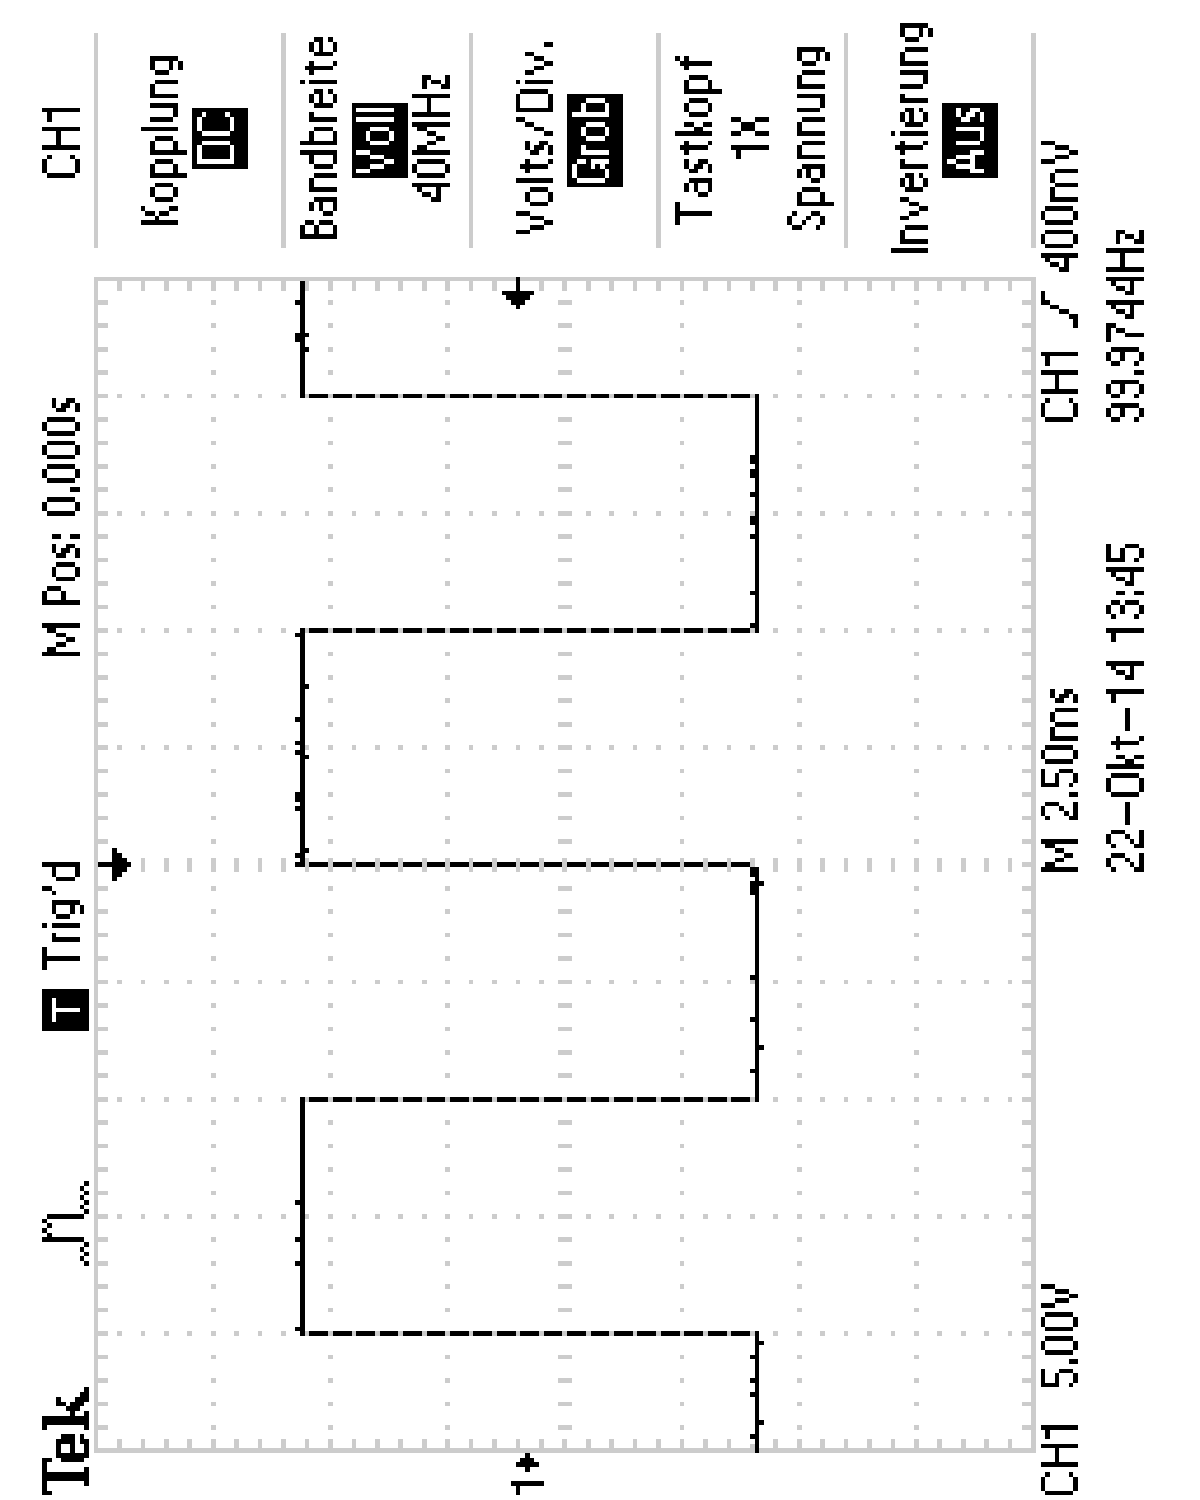
\includegraphics[width=\textwidth , scale = 0.4, angle = -90]{2_1_rech_100hz.pdf}
                \caption[Aufnahme des Rechtecksignals mit einer Frequenz von 100Hz]{Aufnahme des Rechteck Signals mit einer Frequenz von 100Hz}
                \label{fig:2_1_rech_100hz}
        \end{subfigure}%
        ~ %add desired spacing between images, e. g. ~, \quad, \qquad, \hfill etc.
          %(or a blank line to force the subfigure onto a new line)
        \hfill
        \begin{subfigure}[b]{0.28\textwidth}
                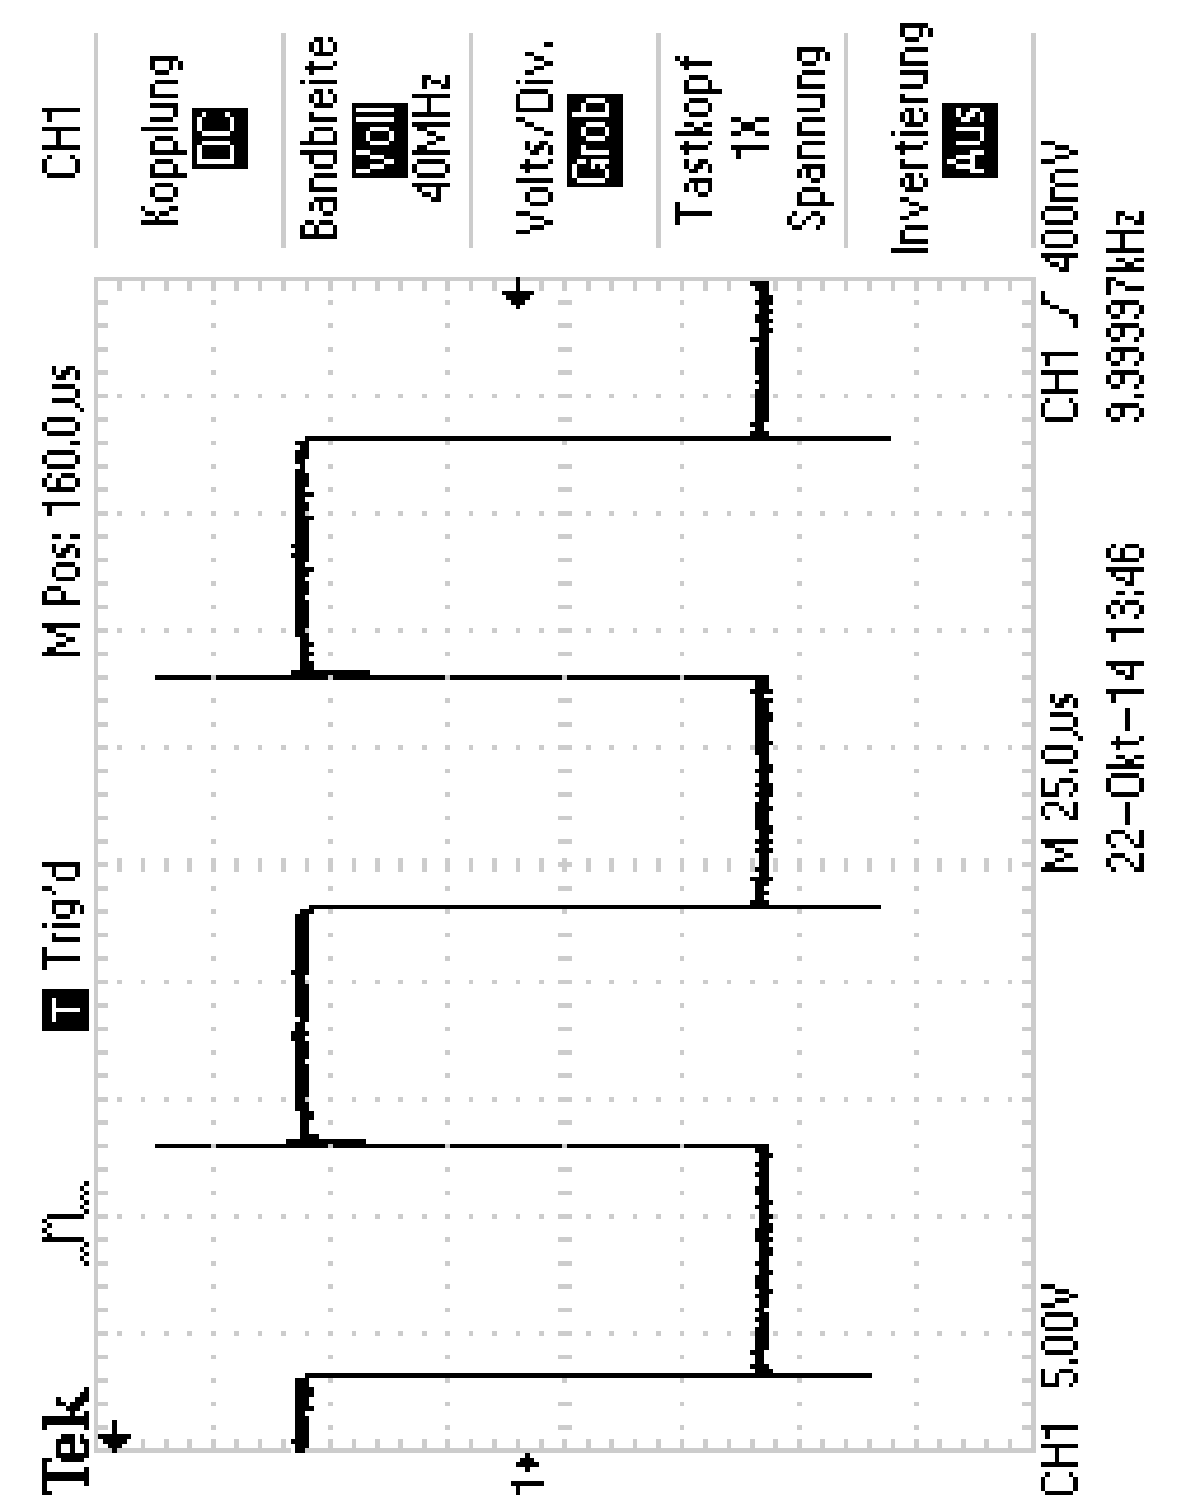
\includegraphics[width=\textwidth , scale = 0.4, angle = -90]{2_1_rech_10khz.pdf}
                \caption[Aufnahme des Rechtecksignals mit einer Frequenz von 10kHz]{Aufnahme des Rechteck Signals mit einer Frequenz von 10kHz}
                \label{fig:2_1_rech_10khz}
        \end{subfigure}
        ~ %add desired spacing between images, e. g. ~, \quad, \qquad, \hfill etc.
          %(or a blank line to force the subfigure onto a new line)
        \hfill
        \begin{subfigure}[b]{0.28\textwidth}
                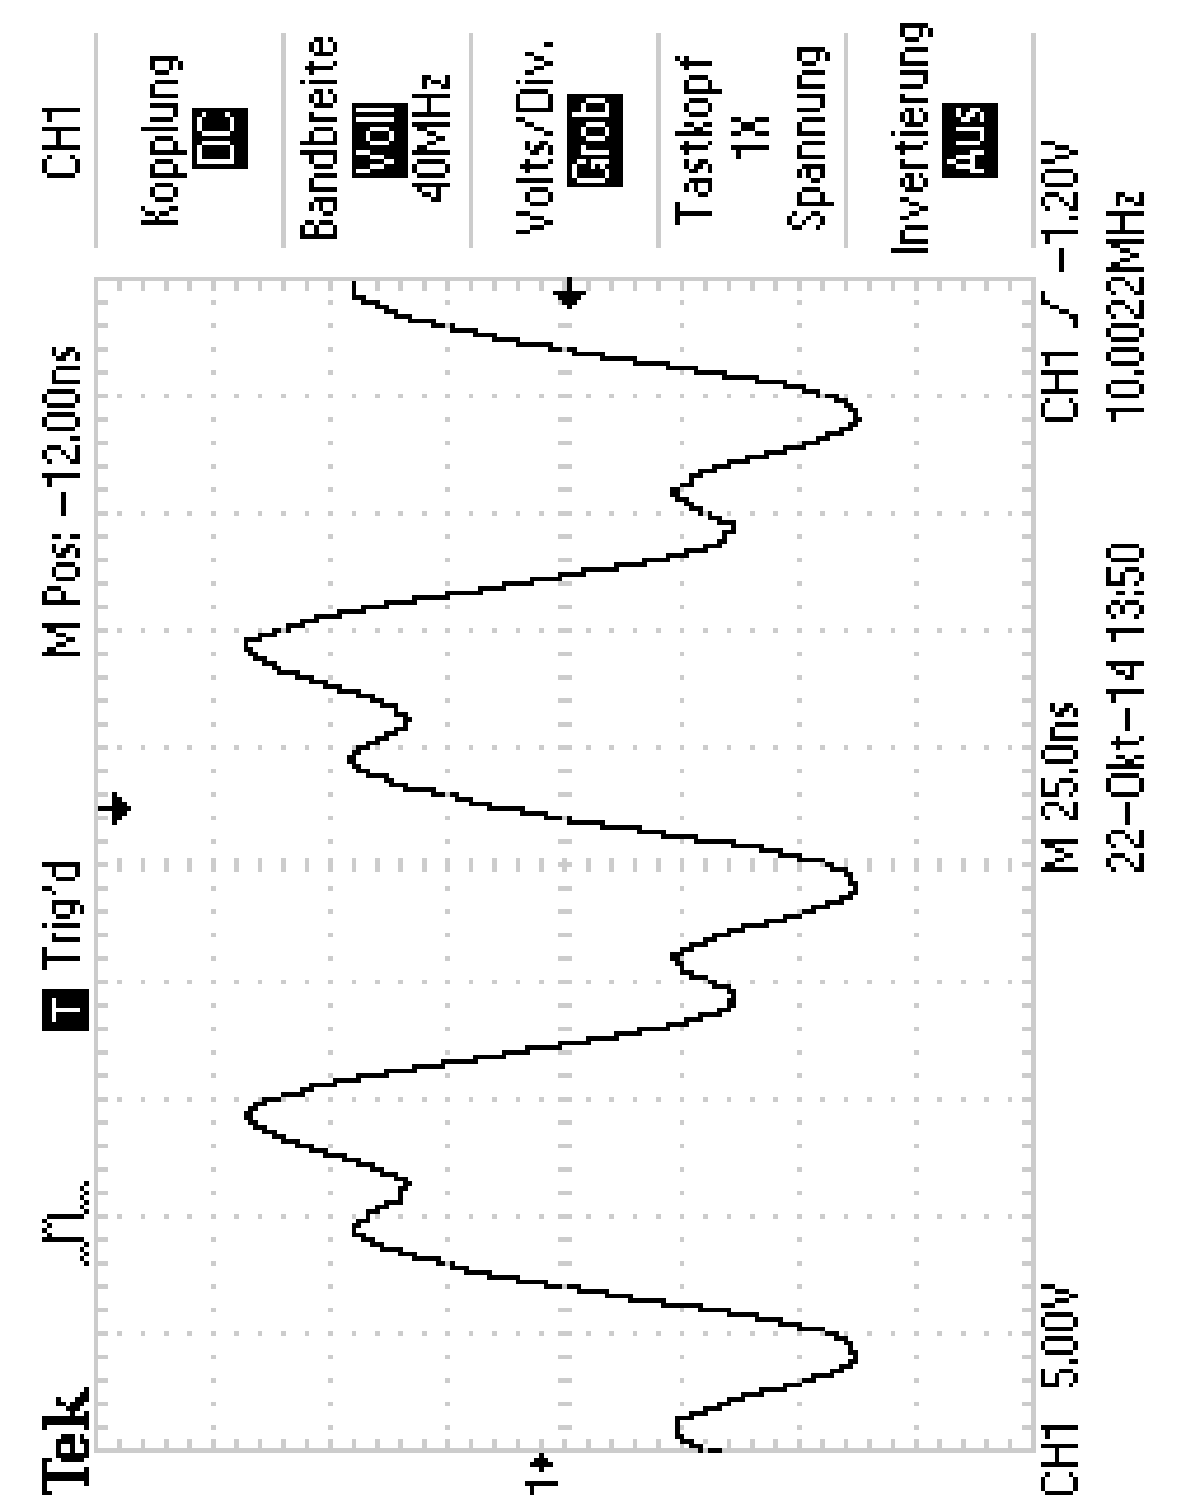
\includegraphics[width=\textwidth , scale = 0.4, angle = -90]{2_1_rech_10mhz.pdf}
                \caption[Aufnahme des Rechtecksignals mit einer Frequenz von 10MHz]{Aufnahme des Rechteck Signals mit einer Frequenz von 10MHz}
  				\label{fig:2_1_rech_10mhz}
        \end{subfigure}
        \caption{Kurve der übertragenen Rechtecksignale für 100Hz,10kHz und 10MHz}
        \label{fig:2_1_rech_vergleich}
\end{figure}



\subsubsection{Versuchsteil 2.2}


Bei der Messung mit zwei Bananenkabeln war die Qualität des Sinussignals bei unterschiedlichen Frequenzen unverändert, was in Abbildung \ref{fig:2_2_sin_vergleich} zu sehen ist.


\begin{figure}[H]
        \centering
        \begin{subfigure}[b]{0.48\textwidth}
                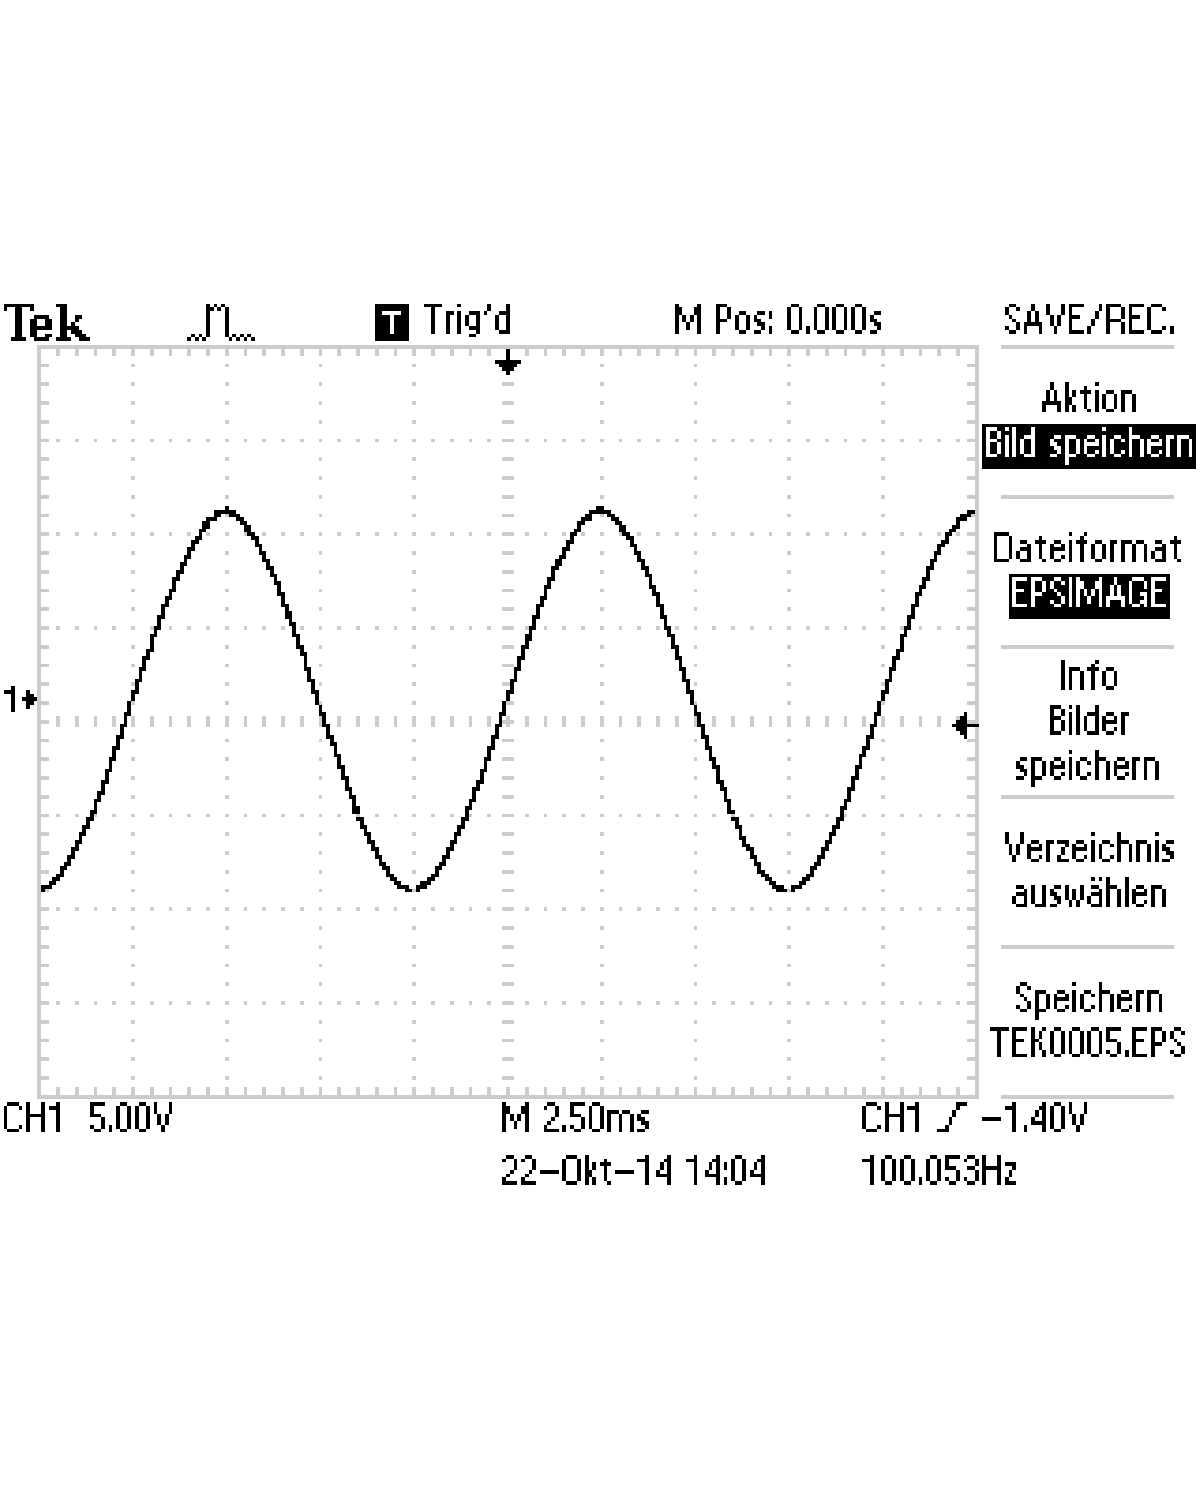
\includegraphics[width=\textwidth , scale = 0.4]{2_2_sin_100hz.pdf}
                \caption[Aufnahme der Sinuswelle mit einer Frequenz von 100Hz]{Aufnahme der Sinuswelle mit einer Frequenz von 100Hz}
 				 \label{fig:2_2_sin_100hz}
        \end{subfigure}%
        ~ %add desired spacing between images, e. g. ~, \quad, \qquad, \hfill etc.
          %(or a blank line to force the subfigure onto a new line)
        \hfill
        \begin{subfigure}[b]{0.48\textwidth}
                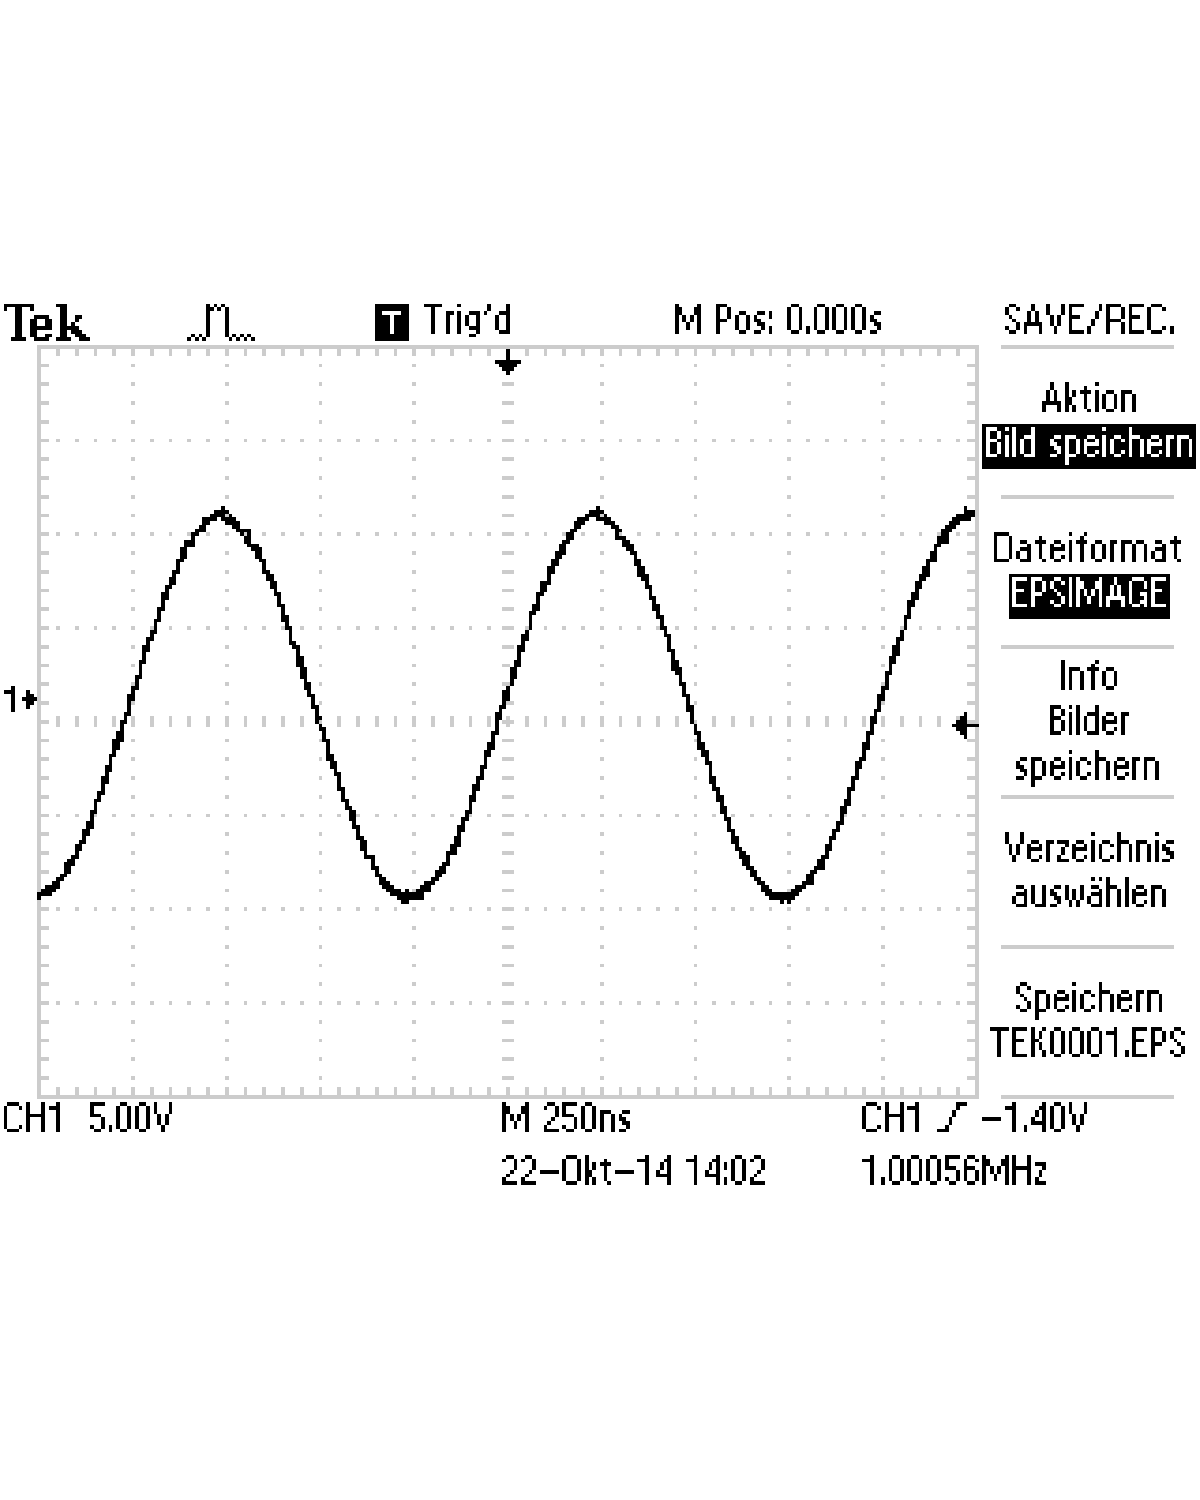
\includegraphics[width=\textwidth , scale = 0.4]{2_2_sin_1mhz.pdf}
                \caption[Aufnahme der Sinuswelle mit einer Frequenz von 1MHz]{Aufnahme der Sinuswelle mit einer Frequenz von 1MHz}
  				\label{fig:2_2_sin_1mhz}
        \end{subfigure}
        \caption{Kurve der übertragenen Sinussignale für 100Hz und 1MHz}
        \label{fig:2_2_sin_vergleich}
\end{figure}

Bei niedriger Frequenz ist das Signal sehr gut zu erkennen, Abbildung \ref{fig:2_2_rech_100hz}.
Die ersten Verzerrungen waren auch wieder bei einer Frequenz von 10kHz zu erkennen, diese fällt jedoch geringer als beim Aufbau zuvor aus, wie in Abbildung \ref{fig:2_2_rech_10khz} zu erkennen ist, was wie zuvor am Anzeigebereich des Oszilloskops liegt.
Bei einer Frequenz von 10MHz ist das vorherige Rechtecksignal als solches wieder nicht mehr zu erkennen. Jedoch ist das Signal deutlich besser erhalten, als bei der einkanaligen Verbindung, wie in Abbildung \ref{fig:2_2_rech_10mhz} zu erkennen ist.


\begin{figure}[H]
        \centering
        \begin{subfigure}[b]{0.28\textwidth}
                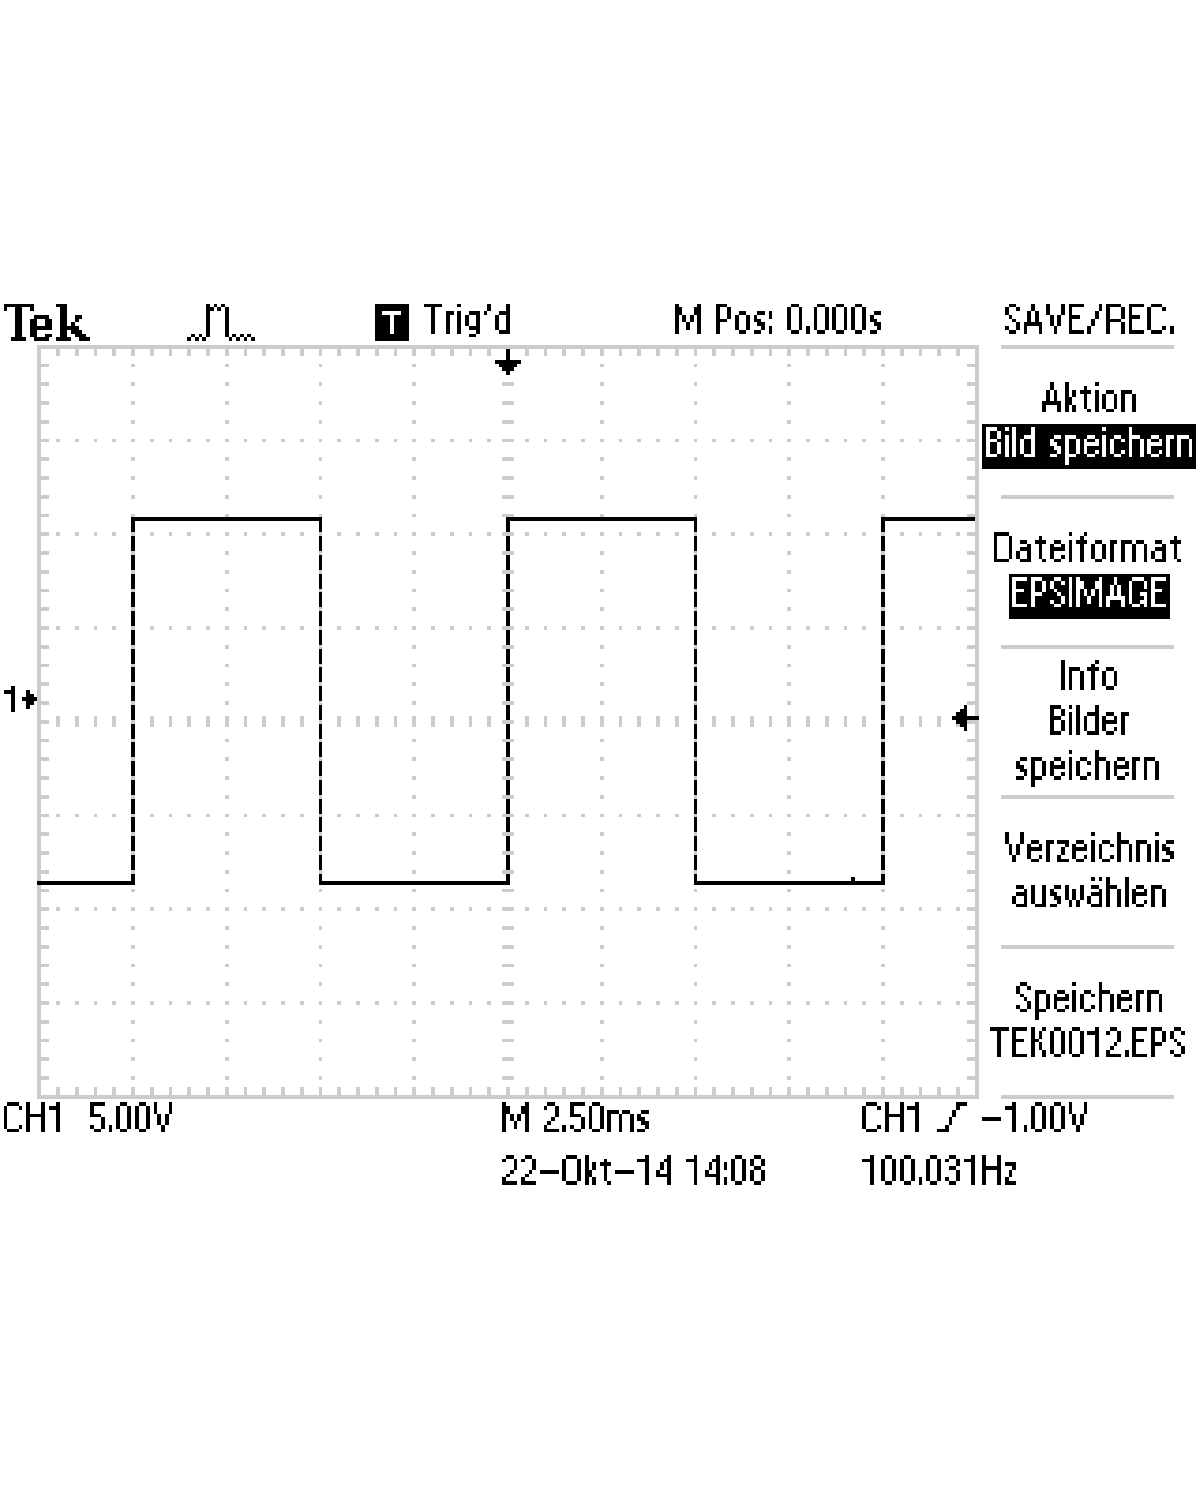
\includegraphics[width=\textwidth , scale = 0.4]{2_2_rech_100hz.pdf}
                \caption[Aufnahme des Rechtecksignals mit einer Frequenz von 100Hz]{Aufnahme des Rechteck Signals mit einer Frequenz von 100Hz}
                \label{fig:2_2_rech_100hz}
        \end{subfigure}%
        ~ %add desired spacing between images, e. g. ~, \quad, \qquad, \hfill etc.
          %(or a blank line to force the subfigure onto a new line)
        \hfill
        \begin{subfigure}[b]{0.28\textwidth}
                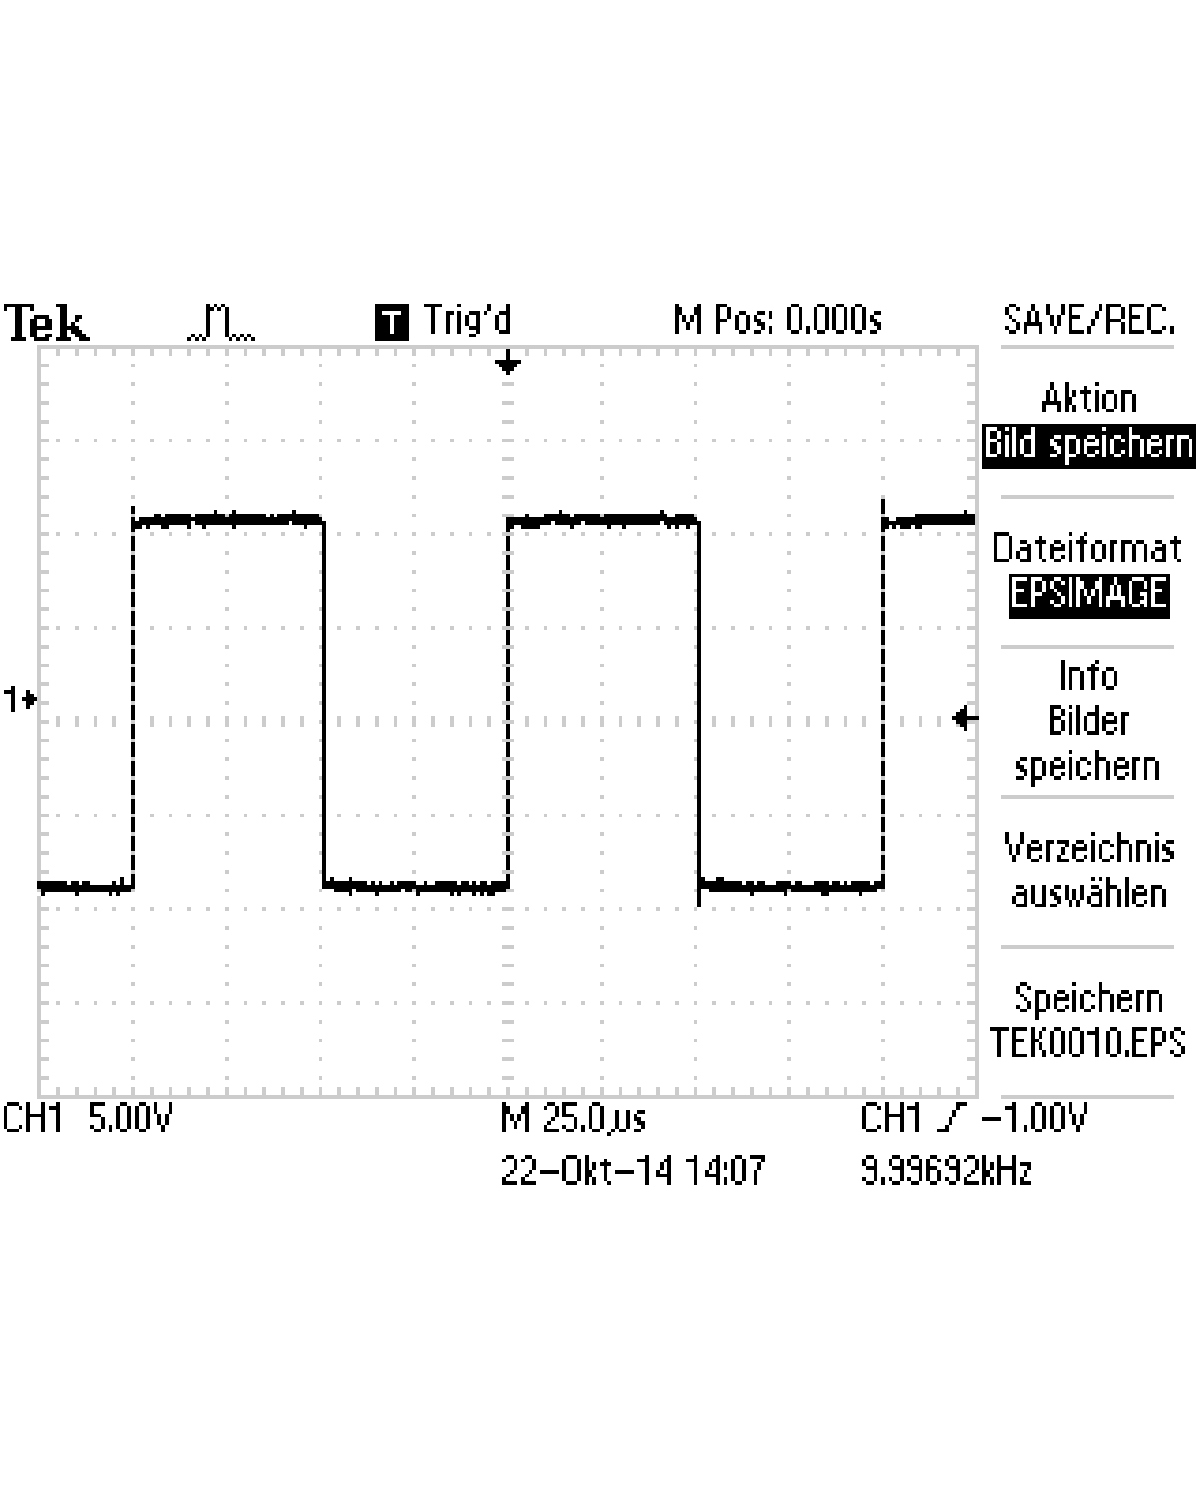
\includegraphics[width=\textwidth , scale = 0.4]{2_2_rech_10khz.pdf}
                \caption[Aufnahme des Rechtecksignals mit einer Frequenz von 10kHz]{Aufnahme des Rechteck Signals mit einer Frequenz von 10kHz}
                \label{fig:2_2_rech_10khz}
        \end{subfigure}
        ~ %add desired spacing between images, e. g. ~, \quad, \qquad, \hfill etc.
          %(or a blank line to force the subfigure onto a new line)
        \hfill
        \begin{subfigure}[b]{0.28\textwidth}
                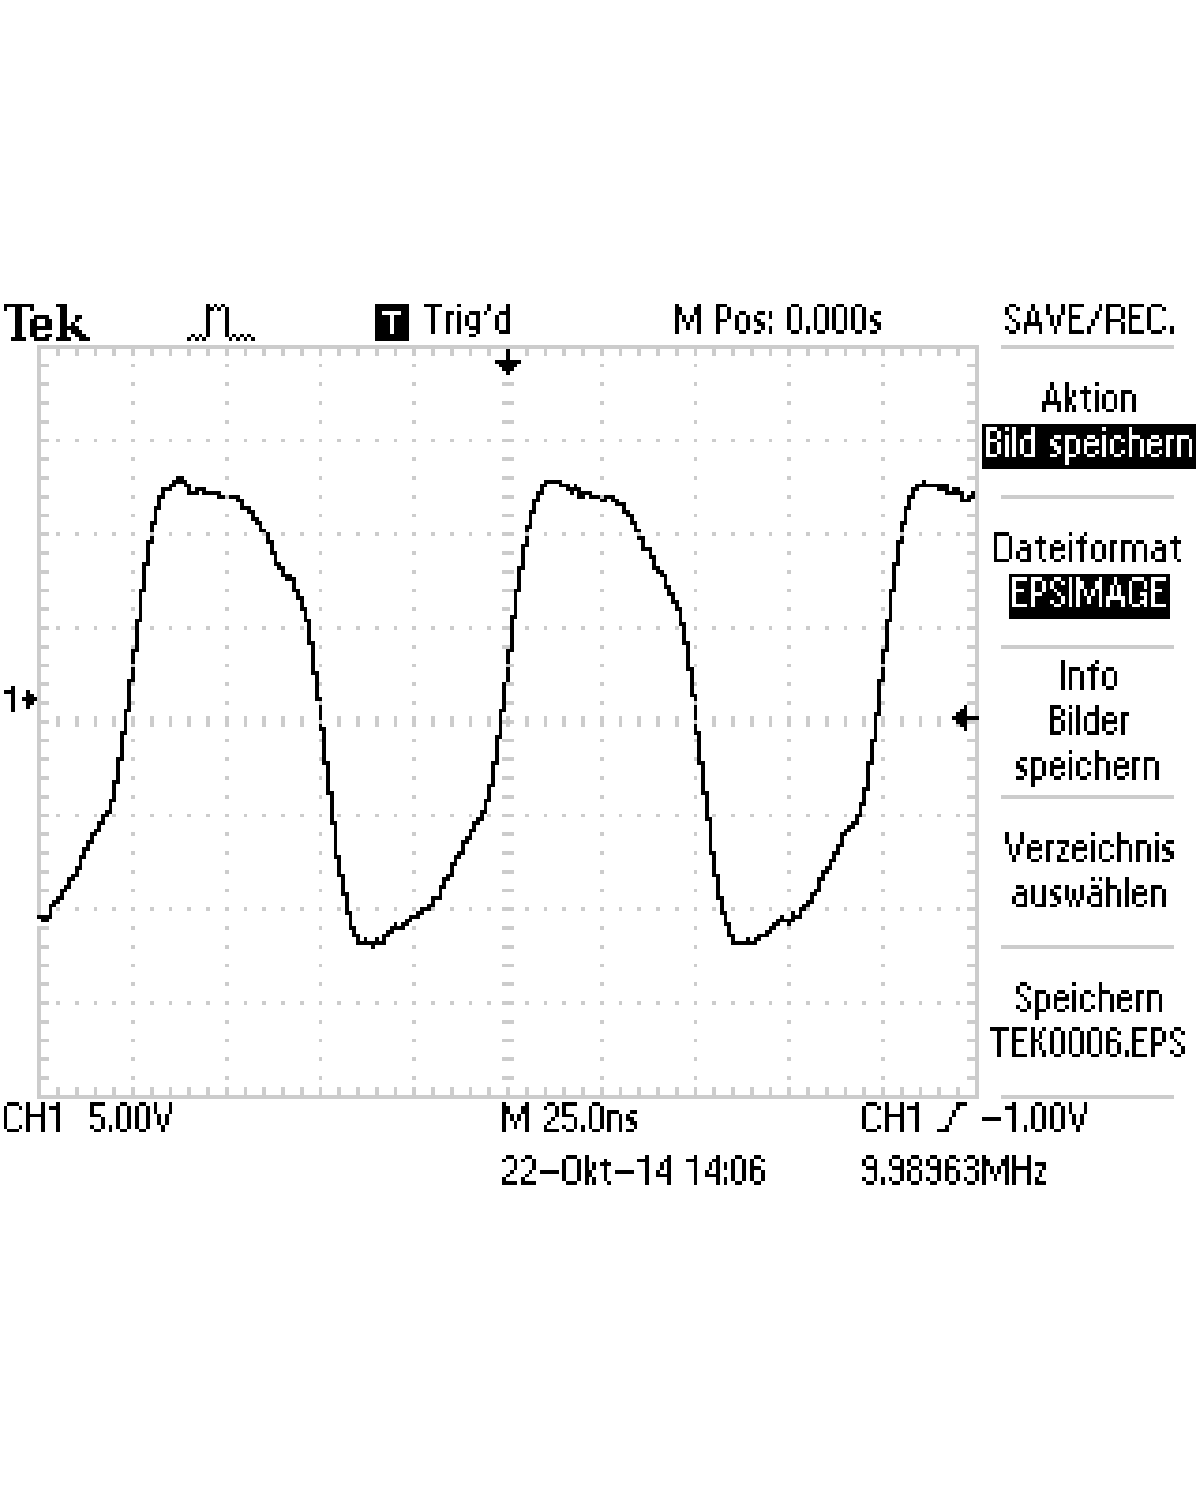
\includegraphics[width=\textwidth , scale = 1]{2_2_rech_10mhz.pdf}
                \caption[Aufnahme des Rechtecksignals mit einer Frequenz von 10MHz]{Aufnahme des Rechteck Signals mit einer Frequenz von 10MHz}
  				\label{fig:2_2_rech_10mhz}
        \end{subfigure}
        \caption{Kurve der übertragenen Rechtecksignale für 100Hz,10kHz und 10MHz}
        \label{fig:2_2_rech_vergleich}
\end{figure}


\subsubsection{Versuchsteil 2.3}

Betrachtet man die Signalübertragung einer Rechteckspannung mit einem twisted-pair Kabel, Abbildung \ref{fig:2_3_vgl_2} und zwei nicht verdrillten Bananenkabeln, Abbildung \ref{fig:2_3_vgl_1} so lässt sich kaum eine Verbesserung feststellen, da die Signalquelle nicht potentialfrei ist.

\begin{figure}[H]
        \centering
        \begin{subfigure}[b]{0.48\textwidth}
                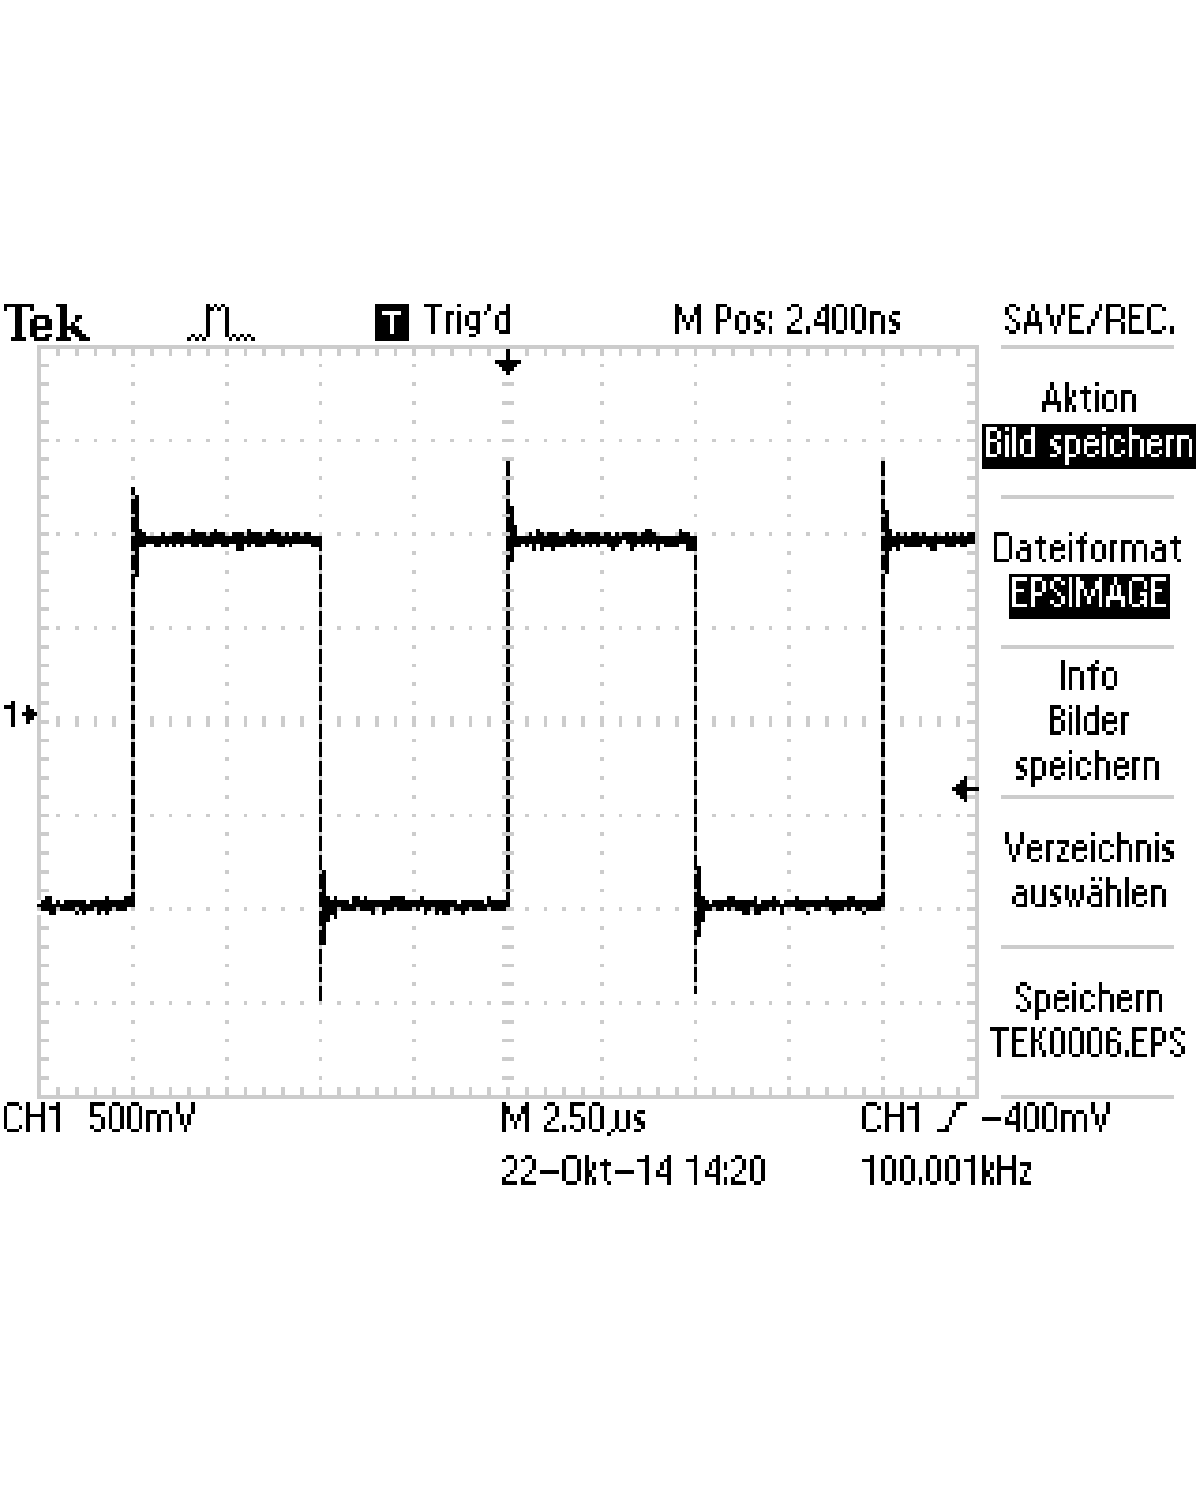
\includegraphics[width=\textwidth , scale = 0.4]{2_3_vgl_2.pdf}
				\caption[Aufnahme des Rechtecksignals, übertragen mit zwei Bananenkabel und einer Frequenz von 100kHz]{Aufnahme des Rechtecksignals, übertragen mit zwei Bananenkabel und einer Frequenz von 100kHz}
 				\label{fig:2_3_vgl_2}
        \end{subfigure}%
        ~ %add desired spacing between images, e. g. ~, \quad, \qquad, \hfill etc.
          %(or a blank line to force the subfigure onto a new line)
        \hfill
        \begin{subfigure}[b]{0.48\textwidth}
                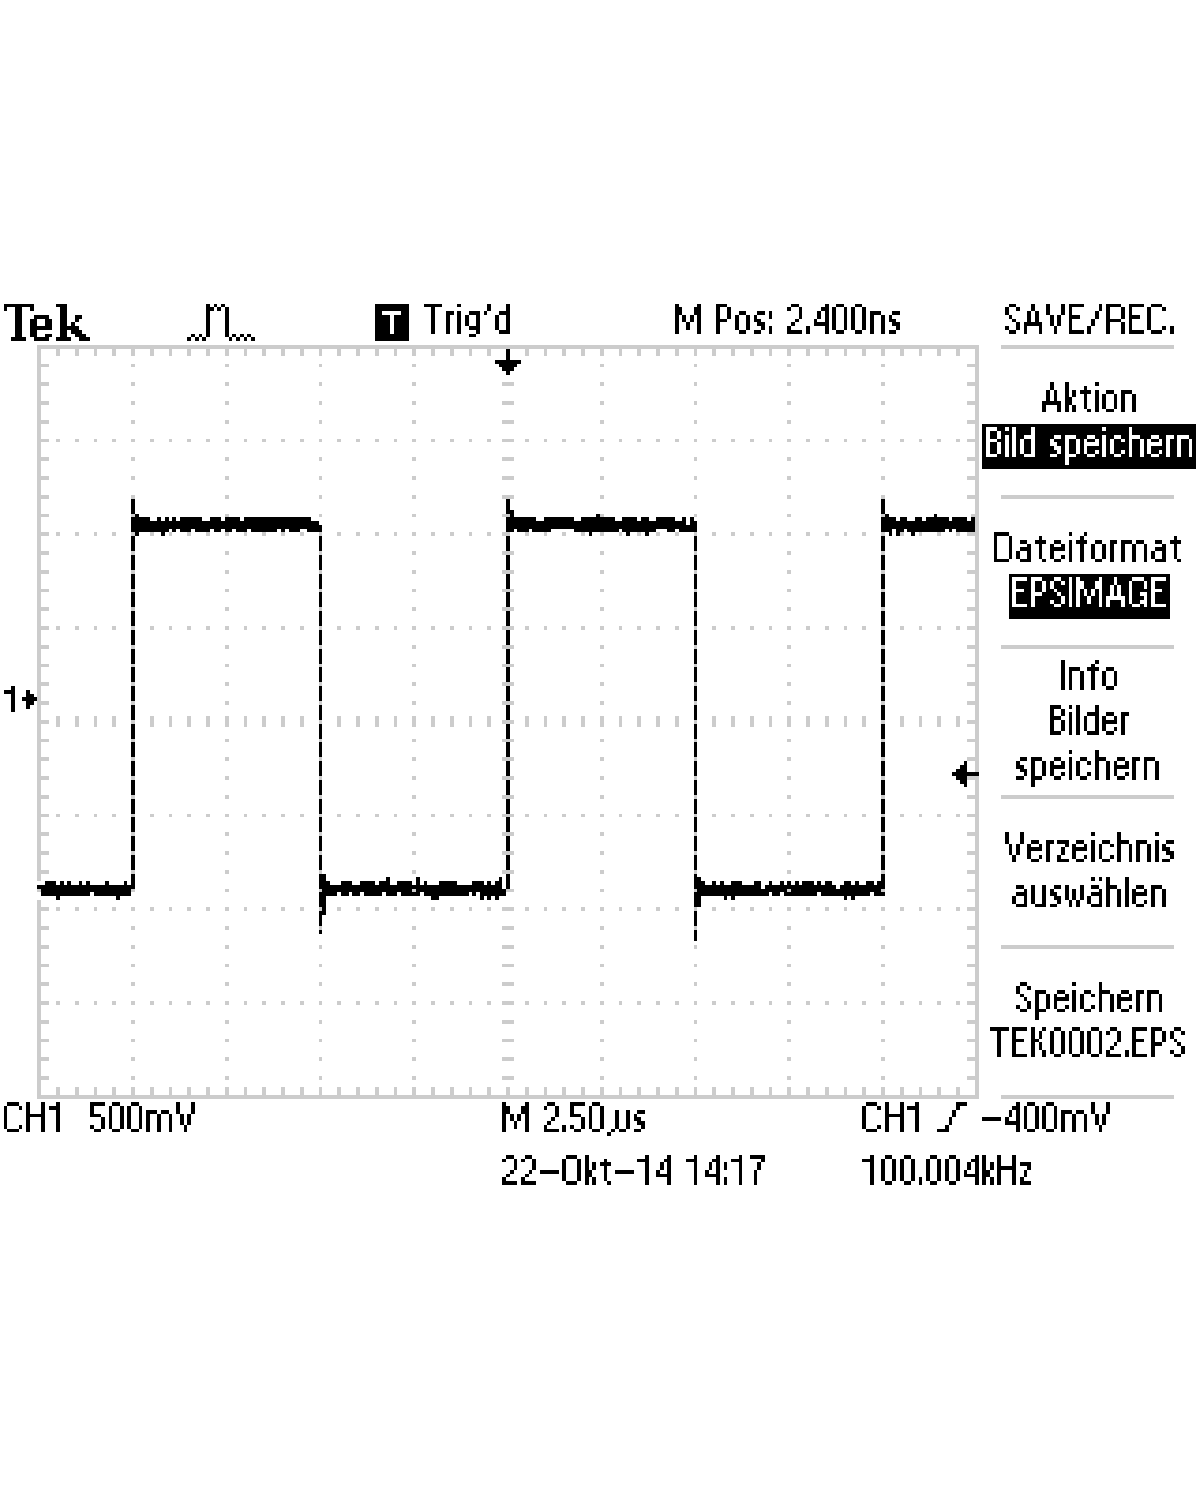
\includegraphics[width=\textwidth , scale = 0.4]{2_3_vgl_1.pdf}
                \caption[Aufnahme des Rechtecksignals, übertragen mit zwei verdrillten Bananenkabel und einer Frequenz von 100kHz]{Aufnahme des Rechtecksignals, übertragen mit zwei verdrillten Bananenkabel und einer Frequenz von 100kHz}
 				\label{fig:2_3_vgl_1}
        \end{subfigure}
        \caption{Kurve der übertragenen Sinussignale für 100Hz und 1MHz}
        \label{fig:2_3_rech_vergleich_ohne_mikro}
\end{figure}


Bei der Messung mit dem Mikrofon ergab sich beim Aufbau nach Abbildung \ref{fig:2.4} die in Abbildung \ref{fig:2_3_r3np_sig} dargestellte Kurve. Für den Aufbau nach Abbildung \ref{fig:2.5} ergab sich die Kurve in Abbildung \ref{fig:2_3_r3p_sig}. Dabei ist zu erkennen, dass die Verschmierung des Signals an den Extrema in Abbildung \ref{fig:2_3_r3p_sig} größer ist als in Abbildung \ref{fig:2_3_r3np_sig}. Dies liegt daran, dass R$_3$ and die Masse angeschlossen ist.
Wenn davon gesprochen wird, dass R$_3$ parallel zu R$_4$ liegt, ist immer auch gemeint, dass R$_3$ an der Masse anliegt.


\begin{figure}[H]
        \centering
        \begin{subfigure}[b]{0.48\textwidth}
                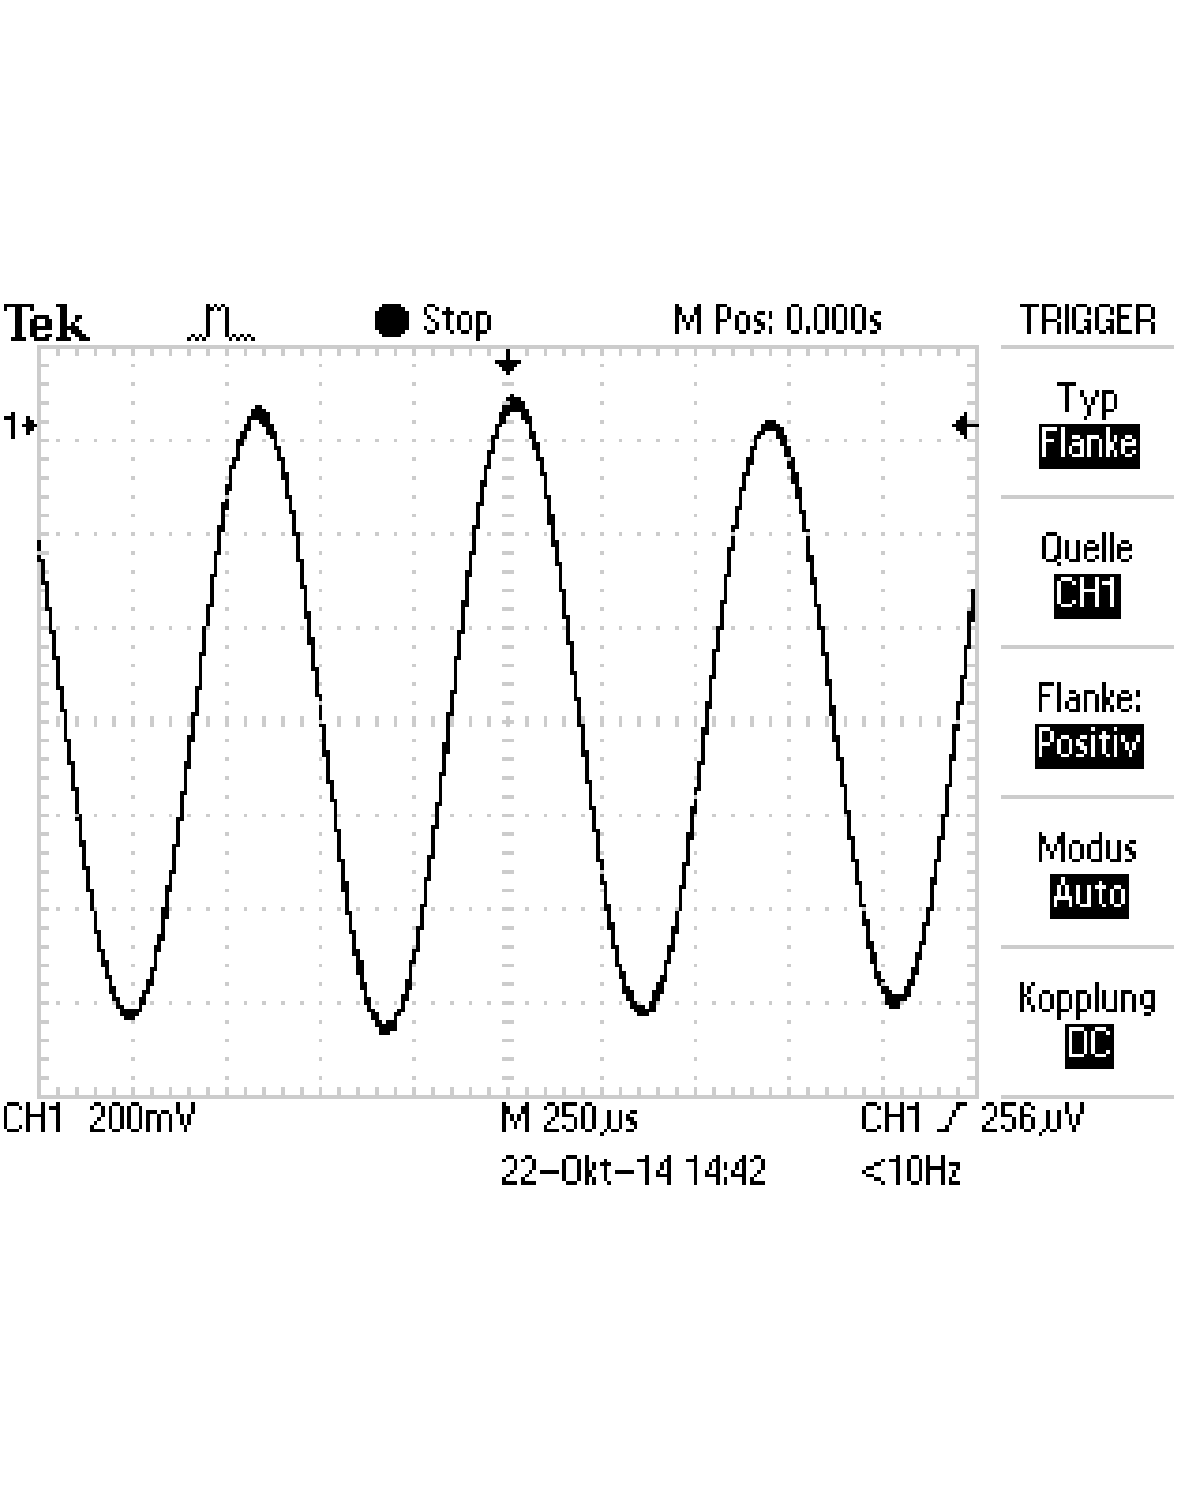
\includegraphics[width=\textwidth , scale = 0.4]{2_3_r3np_sig.pdf}
				\caption[Aufnahme des mit dem Mikrofon aufgenommenen Signals, ohne das R$_3$ parallel zu R$_4$ geschaltet ist]{Aufnahme des mit dem Mikrofon aufgenommenen Signals, ohne das R$_3$ parallel zu R$_4$ geschaltet ist}
  				\label{fig:2_3_r3np_sig}
        \end{subfigure}%
        ~ %add desired spacing between images, e. g. ~, \quad, \qquad, \hfill etc.
          %(or a blank line to force the subfigure onto a new line)
        \hfill
        \begin{subfigure}[b]{0.48\textwidth}
                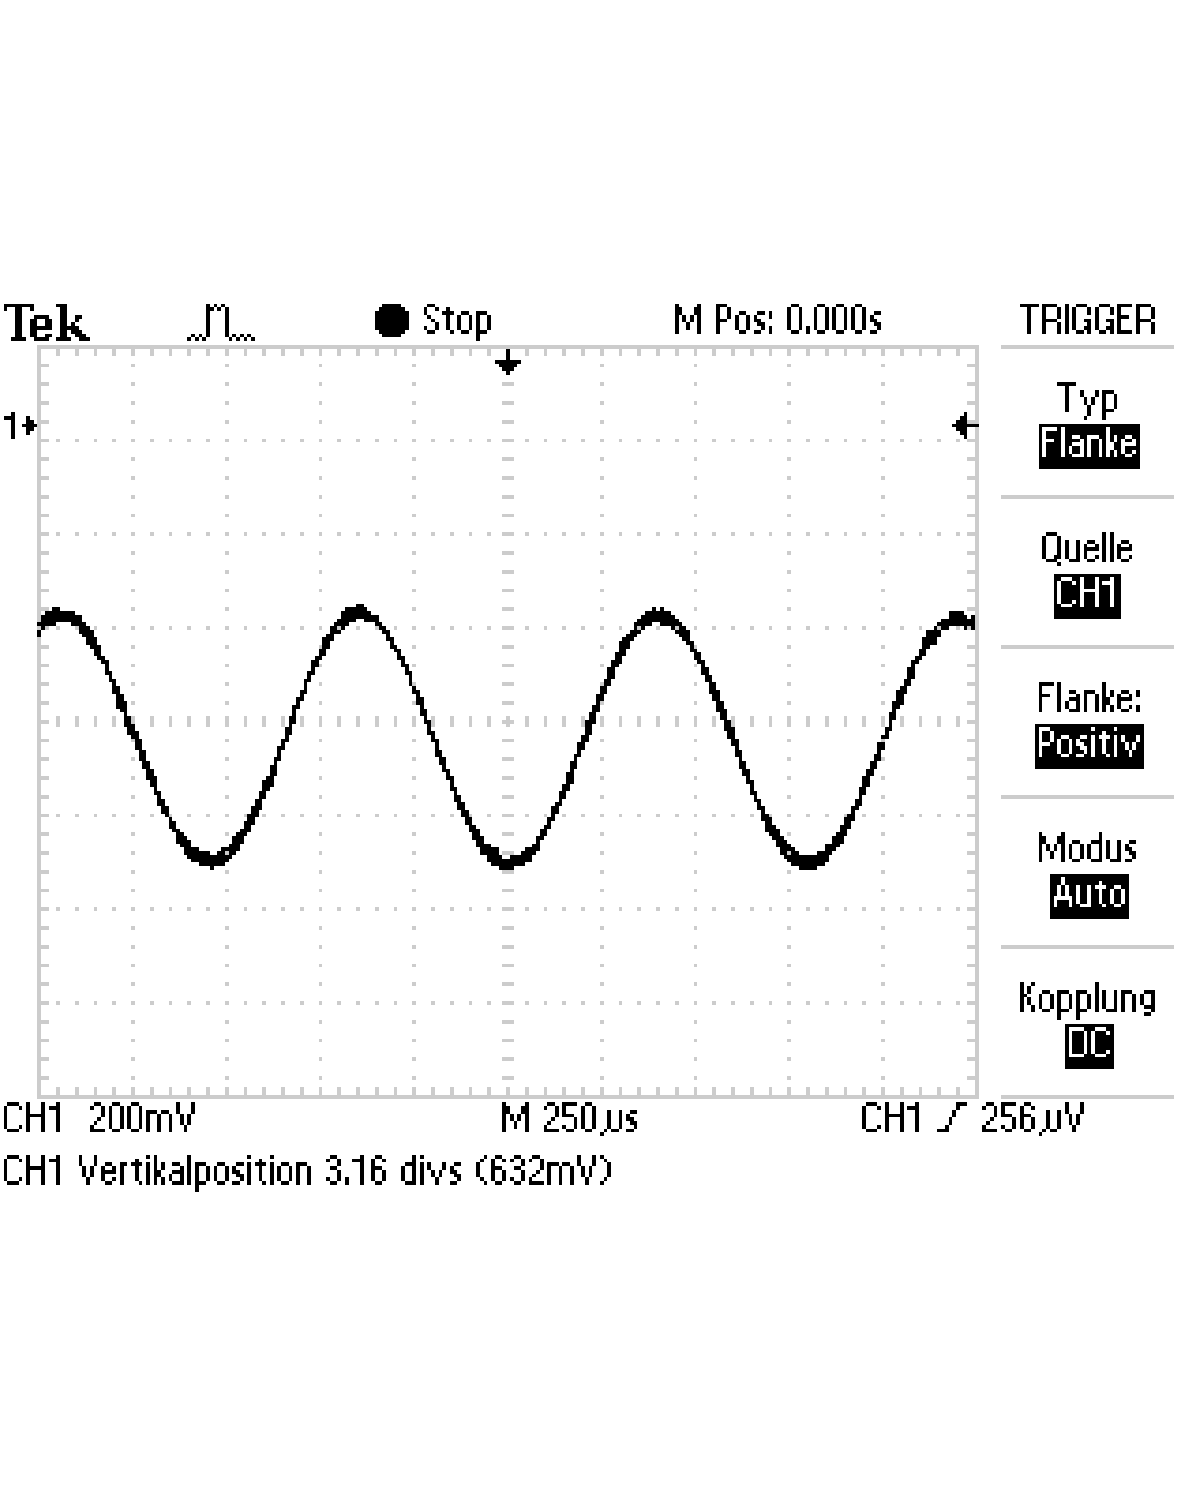
\includegraphics[width=\textwidth , scale = 0.4]{2_3_r3p_sig.pdf}
                \caption[Aufnahme des mit dem Mikrofon aufgenommenen Signals, mit R$_3$ parallel zu R$_4$ geschaltet]{Aufnahme des mit dem Mikrofon aufgenommenen Signals, mit R$_3$ parallel zu R$_4$ geschaltet}
  				\label{fig:2_3_r3p_sig}
        \end{subfigure}
        \caption{Kurven der durch Pfeifen erzeugten Signale}
        \label{fig:2_3_sin_vergleich}
\end{figure}



Betrachtet man die Störung, die dadurch verursacht wird, dass man das Mikrofon auf den Funktionsgenerator legt, so erhält man für R$_3$ nicht parallel zu R$_4$ die Kurve in Abbildung \ref{fig:2_3_r3np_sig}. Für den Aufbau mit R$_3$ parallel zu R$_4$ ergibt sich die Kurve aus Abbildung \ref{fig:2_3_r3p_sig}. Wieder ist zu erkennen, dass die Verschmierung der Kurve aus Abbildung \ref{fig:2_3_r3p_st} größer ist als in Abbildung \ref{fig:2_3_r3np_st}.


\begin{figure}[H]
        \centering
        \begin{subfigure}[b]{0.48\textwidth}
                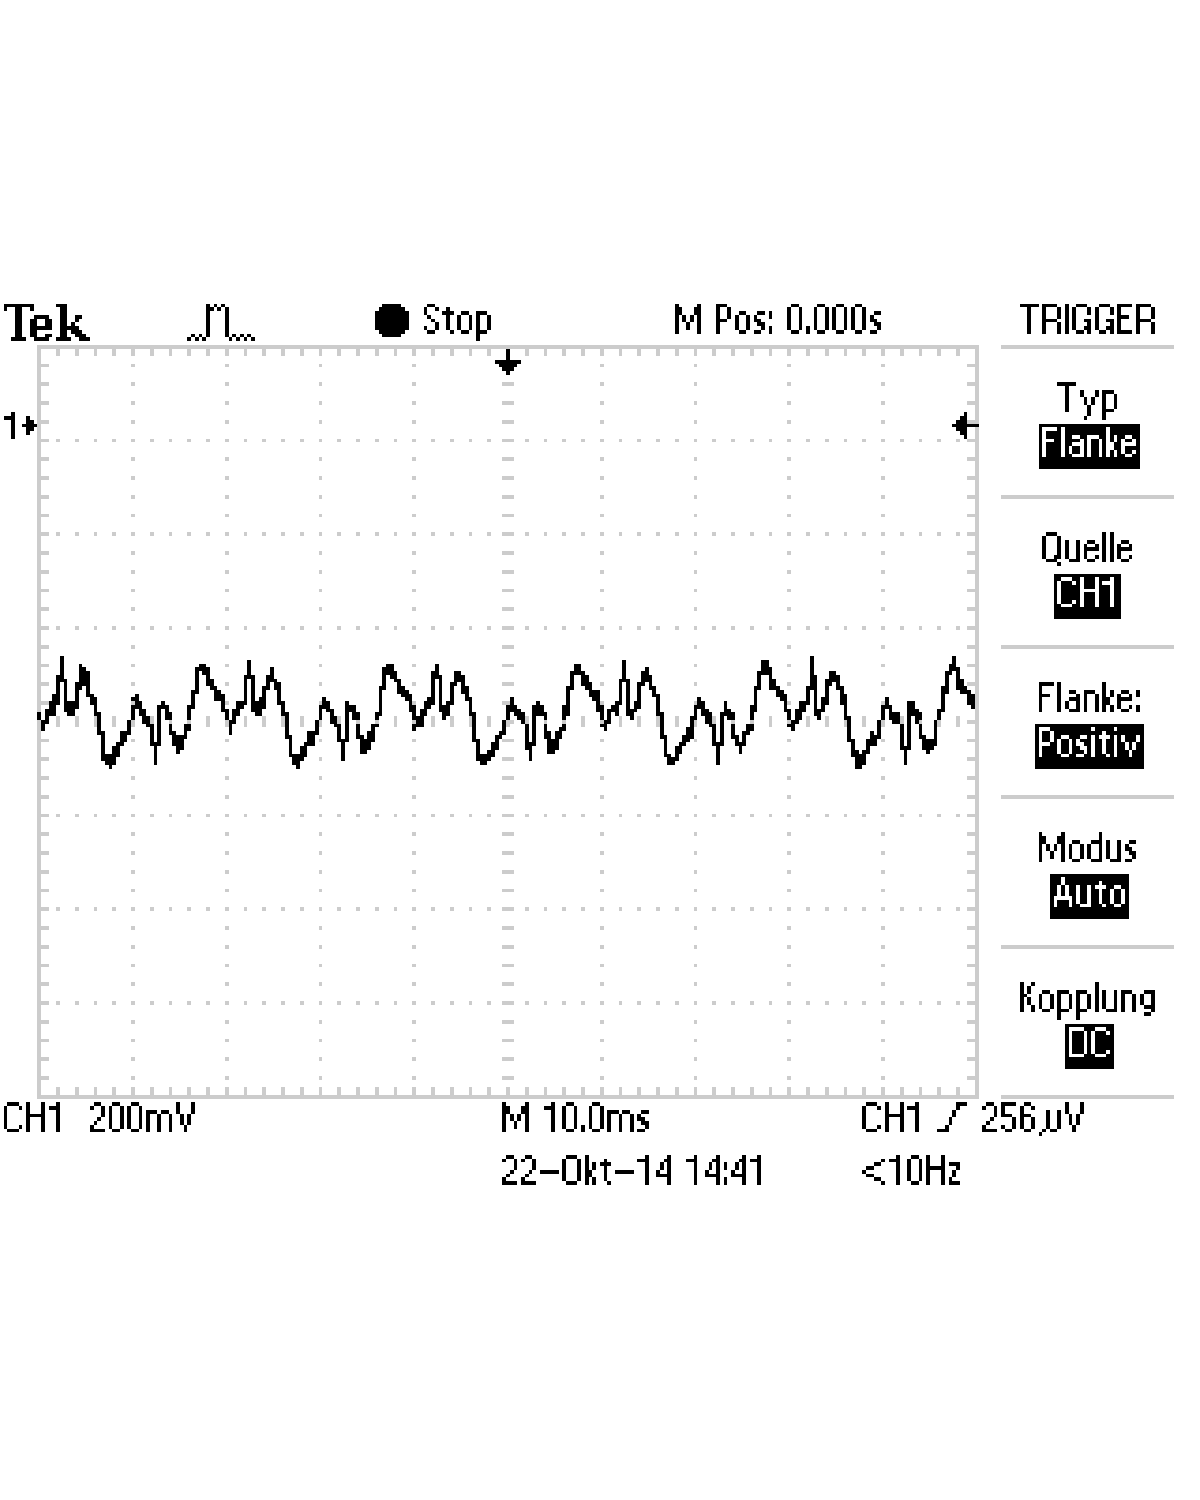
\includegraphics[width=\textwidth , scale = 0.4]{2_3_r3np_st.pdf}
				\caption[Aufnahme der mit dem Mikrofon aufgenommenen Störung, ohne das R$_3$ parallel zu R$_4$ geschaltet ist]{Aufnahme der mit dem Mikrofon aufgenommenen Störung, ohne das R$_3$ parallel zu R$_4$ geschaltet ist}
 	 			\label{fig:2_3_r3np_st}
        \end{subfigure}%
        ~ %add desired spacing between images, e. g. ~, \quad, \qquad, \hfill etc.
          %(or a blank line to force the subfigure onto a new line)
        \hfill
        \begin{subfigure}[b]{0.48\textwidth}
                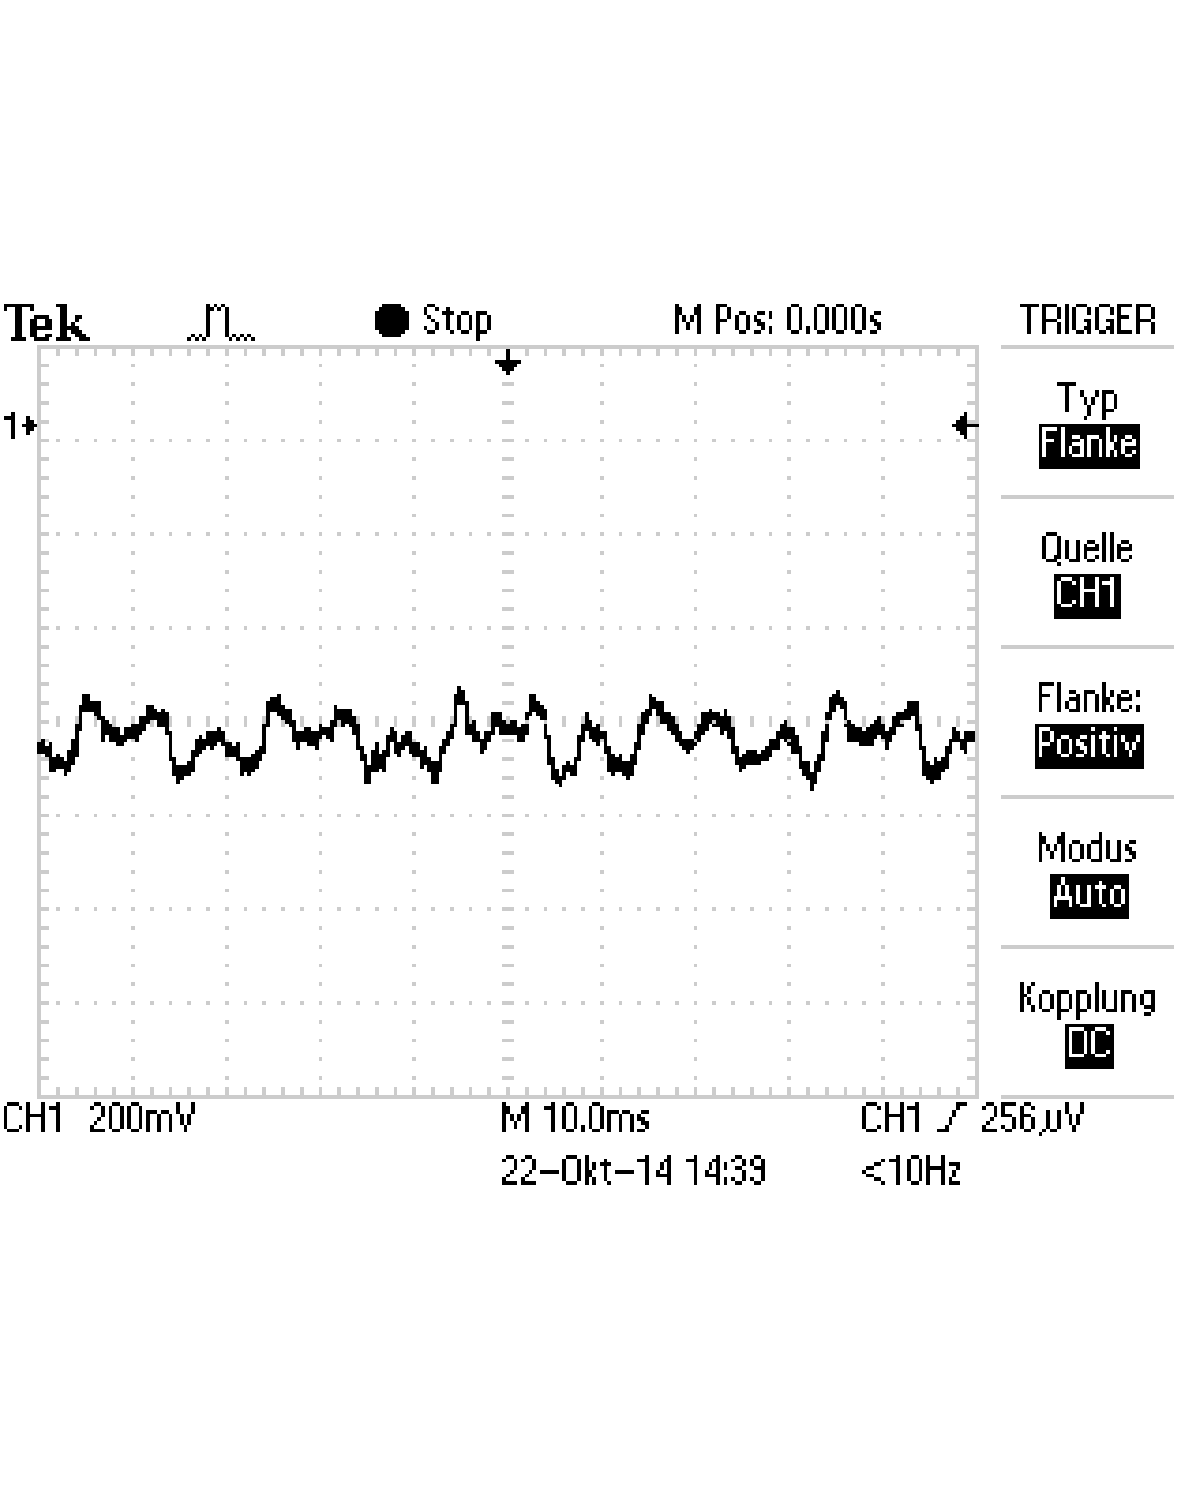
\includegraphics[width=\textwidth , scale = 0.4]{2_3_r3p_st.pdf}
                \caption[Aufnahme der mit dem Mikrofon aufgenommenen Störung, mit R$_3$ parallel zu R$_4$ geschaltet]{Aufnahme der mit dem Mikrofon aufgenommenen Störung, mit R$_3$ parallel zu R$_4$ geschaltet}
  				\label{fig:2_3_r3p_st}
        \end{subfigure}
        \caption{Kurve der Störung durch den Funktionsgenerator}
        \label{fig:2_2_stoer_vergleich}
\end{figure}



\subsection{Diskussion}
%(immer) die gemessenen werte und die bestimmten werte über die messfehler mit literaturwerten oder untereinander vergleichen
%in welchem fehlerintervall des messwertes liegt der literaturwert oder der vergleichswert?
%wie ist der relative anteil des fehlers am messwert und damit die qualität unserer messung?
%in einem satz erklären, wie gut unser fehler und damit unsere messung ist
%kurz erläutern, wie systematische fehler unsere messung beeinflusst haben könnten
%(wichtig) zum schluss ansprechen, in wie weit die ergebnisse mit der theoretischen vorhersage übereinstimmen
%--------------------------------------------------------------------------------------------
%falls tabellen mit den messwerten zu lang werden, kann die section mit den messwerten auch hinter der diskussion angefügt bzw. eine section mit dem anhang eingefügt werden.

Wie erwartet ergab sich bei der Verwendung von zwei Bananenkabeln im Gegensatz zu einem Bananenkabel nur eine leichte Verbesserung, da die Erdung von Funktionsgenerator und Oszilloskop jeweils nur einen geringen Gegenstrom zuließen (vgl Abbildung \ref{fig:2_1_rech_vergleich} und Abbildung \ref{fig:2_2_rech_vergleich}).
Da dies auch für die zwei verdrillten Bananenkabel gilt ließen sich bei der Verwendung auch keine Verbesserung beobachten, Abbildung \ref{fig:2_3_rech_vergleich_ohne_mikro}. Beim Verwenden des Mikrofons als Signalquelle lies sich eine leichte Verbesserung feststellen, wenn R$_3$ nicht parallel zu R$_4$ geschaltet war, Abbildung \ref{fig:2_3_sin_vergleich} und Abbildung \ref{fig:2_2_stoer_vergleich}.



\section{Fazit}
%im fazit nochmal alles zusammenfassen und den verlauf der messung abschätzen
%gravierende sytematische probleme bei den messungen nochmal betonen und die wertigkeit unserer ergebnisse einordnen

\end{document}

